% =============================================================================
%  Simulation section — stand-alone fragment for inclusion in main CogSci paper
%  Compile as standalone:  pdflatex simulation_standalone.tex
%  Include in main paper:  % =============================================================================
%  Simulation section — stand-alone fragment for inclusion in main CogSci paper
%  Compile as standalone:  pdflatex simulation_standalone.tex
%  Include in main paper:  % =============================================================================
%  Simulation section — stand-alone fragment for inclusion in main CogSci paper
%  Compile as standalone:  pdflatex simulation_standalone.tex
%  Include in main paper:  % =============================================================================
%  Simulation section — stand-alone fragment for inclusion in main CogSci paper
%  Compile as standalone:  pdflatex simulation_standalone.tex
%  Include in main paper:  \input{simulation}
% =============================================================================

\section{Simulation}

\subsection{Overview}

A factorial simulation examined how two RSA speaker architectures and two
semantic regimes jointly determine the size-first advantage.
The speaker factor crosses an \textit{incremental} speaker that composes
utterances token-by-token via a chain rule with a \textit{global} speaker
that evaluates full two-word utterances at once.
The semantics factor crosses \textit{recursive} semantics, in which the
size threshold adapts to the listener's running posterior at each
composition step, with \textit{static} semantics, in which the threshold is
computed once from the uniform prior and held fixed.
The central measure is communicative success: the probability that a
pragmatic listener, reasoning about the speaker, recovers the intended
referent from a given utterance.
Size-first (\textit{big blue}) is taken to be preferred whenever it yields
strictly higher communicative success than color-first (\textit{blue big}).

\subsection{Model}

\paragraph{Referents and contexts.}
Each context consists of $n_{\text{obj}}$ objects drawn from a
log-normal size distribution with spread parameter $\sigma_{\text{sd}}$,
with each draw independently assigned a uniformly random color (0 or 1) and
form (0 or 1).
The intended referent is always the object with the largest size, color
$= 1$ (``blue''), and form $= 1$.
The uniform object prior is $P(s) = 1/n_{\text{obj}}$.

\paragraph{Adjective semantics.}
For a color adjective (``blue''),
\begin{equation}
  \llbracket \text{blue} \rrbracket(s) \;=\;
  c_s \cdot v_c + (1 - c_s)(1 - v_c),
\end{equation}
where $c_s \in \{0,1\}$ is the object's color feature and
$v_c \in (0.5, 1)$ is the color semantic value (how reliably the word
maps to the feature).

For a size adjective (``big''), applicability is modeled as a
cumulative-normal threshold function with perceptual blur $\omega$:
\begin{equation}
  \llbracket \text{big} \rrbracket(s) \;=\;
  \Phi\!\left(\frac{s - \theta}{\omega\sqrt{s^2 + \theta^2}}\right),
\end{equation}
where $\theta$ is a context-sensitive threshold and
$\omega$ controls sharpness: small $\omega$ produces a steep CDF
so that only the very largest object receives high applicability.

\paragraph{Threshold.}
The threshold $\theta$ is defined over the mid-range of the context
distribution $C$,
\begin{equation}
  \theta_k(C) \;=\;
  x_{\max}^{\text{mid}}(C) - k\bigl(x_{\max}^{\text{mid}}(C) - x_{\min}^{\text{mid}}(C)\bigr),
\end{equation}
where $x_{\min}^{\text{mid}}$ and $x_{\max}^{\text{mid}}$ are the
20th- and 80th-percentile sizes in $C$, and $k \in [0,1]$ shifts
the threshold between the top and the middle of the mid-range.
Higher $k$ lowers the threshold, admitting more objects as ``big.''

\paragraph{Literal listener.}
For single-word utterances,
$L_0(s \mid w) \propto \llbracket w \rrbracket(s) \cdot P(s)$.
For two-word utterances $u = w_1 w_2$, the literal listener applies
backward functional composition, processing tokens right-to-left and
updating the posterior at each step.
Under \textit{recursive} semantics, the size threshold $\theta$ is
recomputed from this running posterior before each token is applied, so the
threshold adapts to the listener's evolving belief state.
Under \textit{static} semantics, $\theta$ is computed once from the uniform
prior and held fixed throughout composition.
In both cases the final result is
$L_0(s \mid w_1 w_2) \propto
  \llbracket w_1 \rrbracket(s) \cdot \llbracket w_2 \rrbracket(s) \cdot P(s)$,
but under recursive semantics the semantic values of the size adjective
differ between the two orderings because the threshold depends on which
token was processed first.

\paragraph{Global speaker.}
The global speaker evaluates both full two-word utterances simultaneously,
\begin{equation}
  S_G(u \mid s) \;\propto\; \bigl[L_0(s \mid u)\bigr]^\alpha,
  \quad u \in \{\text{big-blue},\; \text{blue-big}\},
\end{equation}
treating each ordering as an atomic unit.

\paragraph{Incremental speaker.}
The incremental speaker applies a two-step chain rule
following \citeA{cohn-gordon-et-al2019}.
At step 1, it selects a first token by reasoning over the single-word
literal listener:
\begin{equation}
  S_1(w_1 \mid s)
    \;\propto\; \bigl[L_0(s \mid w_1)\bigr]^\alpha.
\end{equation}
At step 2, given prefix $w_1$, it decides whether to continue:
\begin{equation}
  S_2(w_2 \mid w_1, s)
    \;\propto\; \bigl[L_0(s \mid w_1 w_2)\bigr]^\alpha,
\end{equation}
where the alternative is stopping at the single word $w_1$.
The full utterance probability is then
\begin{equation}
  S_I(w_1 w_2 \mid s) \;=\; S_1(w_1 \mid s) \cdot S_2(w_2 \mid w_1, s).
  \label{eq:inc-chain}
\end{equation}

\paragraph{Pragmatic listener.}
The pragmatic listener inverts the speaker distribution via Bayes' rule
with a uniform prior over referents,
\begin{equation}
  L_1(s \mid u) \;\propto\; S(u \mid s) \cdot P(s).
\end{equation}
The primary dependent variable is the \textit{size-first advantage},
\begin{equation}
  \Delta(s) \;=\;
  L_1(s^* \mid \text{big-blue}) - L_1(s^* \mid \text{blue-big}),
\end{equation}
where $s^*$ is the intended referent.
Positive values indicate that the size-first order yields higher
communicative success.

\subsection{Parameter Sweep}

Seven parameters were varied factorially (Table~\ref{tab:params}).
For each combination, 1{,}000 contexts were sampled, yielding
12{,}000{,}000 rows total.
The simulation was implemented in JAX \citep{jax2018github} and executed
in a single vectorized pass using nested \texttt{vmap}/\texttt{jit},
completing in under 90 seconds on CPU.

\begin{table}[h]
\centering
\small
\caption{Simulation parameter grid.}
\label{tab:params}
\begin{tabular}{llc}
\toprule
Parameter & Values & $n$ \\
\midrule
$n_{\text{obj}}$    & 2, 6, 10, 14, 18, 22, 26, 30 & 8 \\
Speaker model       & incremental, global           & 2 \\
Semantics           & recursive, static             & 2 \\
$v_c$ (color sem.)  & 0.90, 0.92, 0.94, 0.96, 0.98 & 5 \\
$k$ (threshold)     & 0.1, 0.3, 0.5, 0.7, 0.9      & 5 \\
$\omega$ (blur)     & 0.1, 0.2, 0.3, 0.5, 0.8      & 5 \\
$\sigma_{\text{sd}}$ (context spread) & 2.0, 7.75, 15.0 & 3 \\
\midrule
\multicolumn{2}{l}{Fixed: $\alpha = 1$, bias $= 0$, utterance length $= 2$} & \\
\bottomrule
\end{tabular}
\end{table}

\subsection{Results}

\subsubsection{Recursive Semantics: Global Speaker}

Under recursive semantics, the global speaker produced a consistent
size-first advantage across virtually all parameter combinations.
Averaging over all contexts and parameter values, it assigned
$L_1(s^* \mid \text{big-blue}) = 0.138$ versus
$L_1(s^* \mid \text{blue-big}) = 0.122$,
yielding a mean advantage of $\Delta = +0.016$.
Across individual parameter combinations, 64.8\% produced a positive
advantage, and the direction was preserved across all levels of
$n_{\text{obj}}$, $\sigma_{\text{sd}}$, and $v_c$.

The preference arises because, under recursive semantics, the size
threshold shifts when ``big'' versus ``blue'' is processed first.
This asymmetry in the literal listener makes the two orderings
non-equivalent, and the global speaker exploits the ordering that
maximizes referent recovery.

\subsubsection{Recursive Semantics: Incremental Speaker}

Under recursive semantics, the incremental speaker showed a qualitatively
different pattern depending on the perceptual blur parameter $\omega$.
At $\omega = 0.5$ (the default in prior work), the incremental speaker
produced a \textit{negative} mean advantage ($\Delta = -0.016$),
with only 23.7\% of parameter combinations favoring size-first.
This reversal reflects a structural asymmetry in the chain rule
(Equation~\ref{eq:inc-chain}):
The referent is by construction the only object with color $= 1$, so
$\llbracket \text{blue} \rrbracket(s^*)$ is close to $v_c$ ($\approx 0.90$--$0.98$)
while $\llbracket \text{blue} \rrbracket(s)$ for any non-referent is close to
$1 - v_c$ ($\approx 0.02$--$0.10$).
The color adjective thus almost perfectly identifies the referent at
step~1.
The size adjective, however, depends on $\omega$: at large $\omega$,
the CDF is shallow and multiple objects receive moderate size
applicability, reducing the discriminating power of ``big'' relative to
``blue.''
When ``blue'' is the more informative first token, the incremental
speaker prefers to say it first, producing \textit{blue big}.

Reducing $\omega$ sharpens the size CDF so that only the largest object
receives high applicability, restoring size as a reliable discriminator at
step~1.
Figure~\ref{fig:adv-wf} shows a monotone relationship between $\omega$
and $\Delta$ for the incremental speaker: the size-first advantage crosses
zero at approximately $\omega \approx 0.30$, and reaches a mean of
$+0.049$ at $\omega = 0.1$.

\begin{figure}[h]
  \centering
  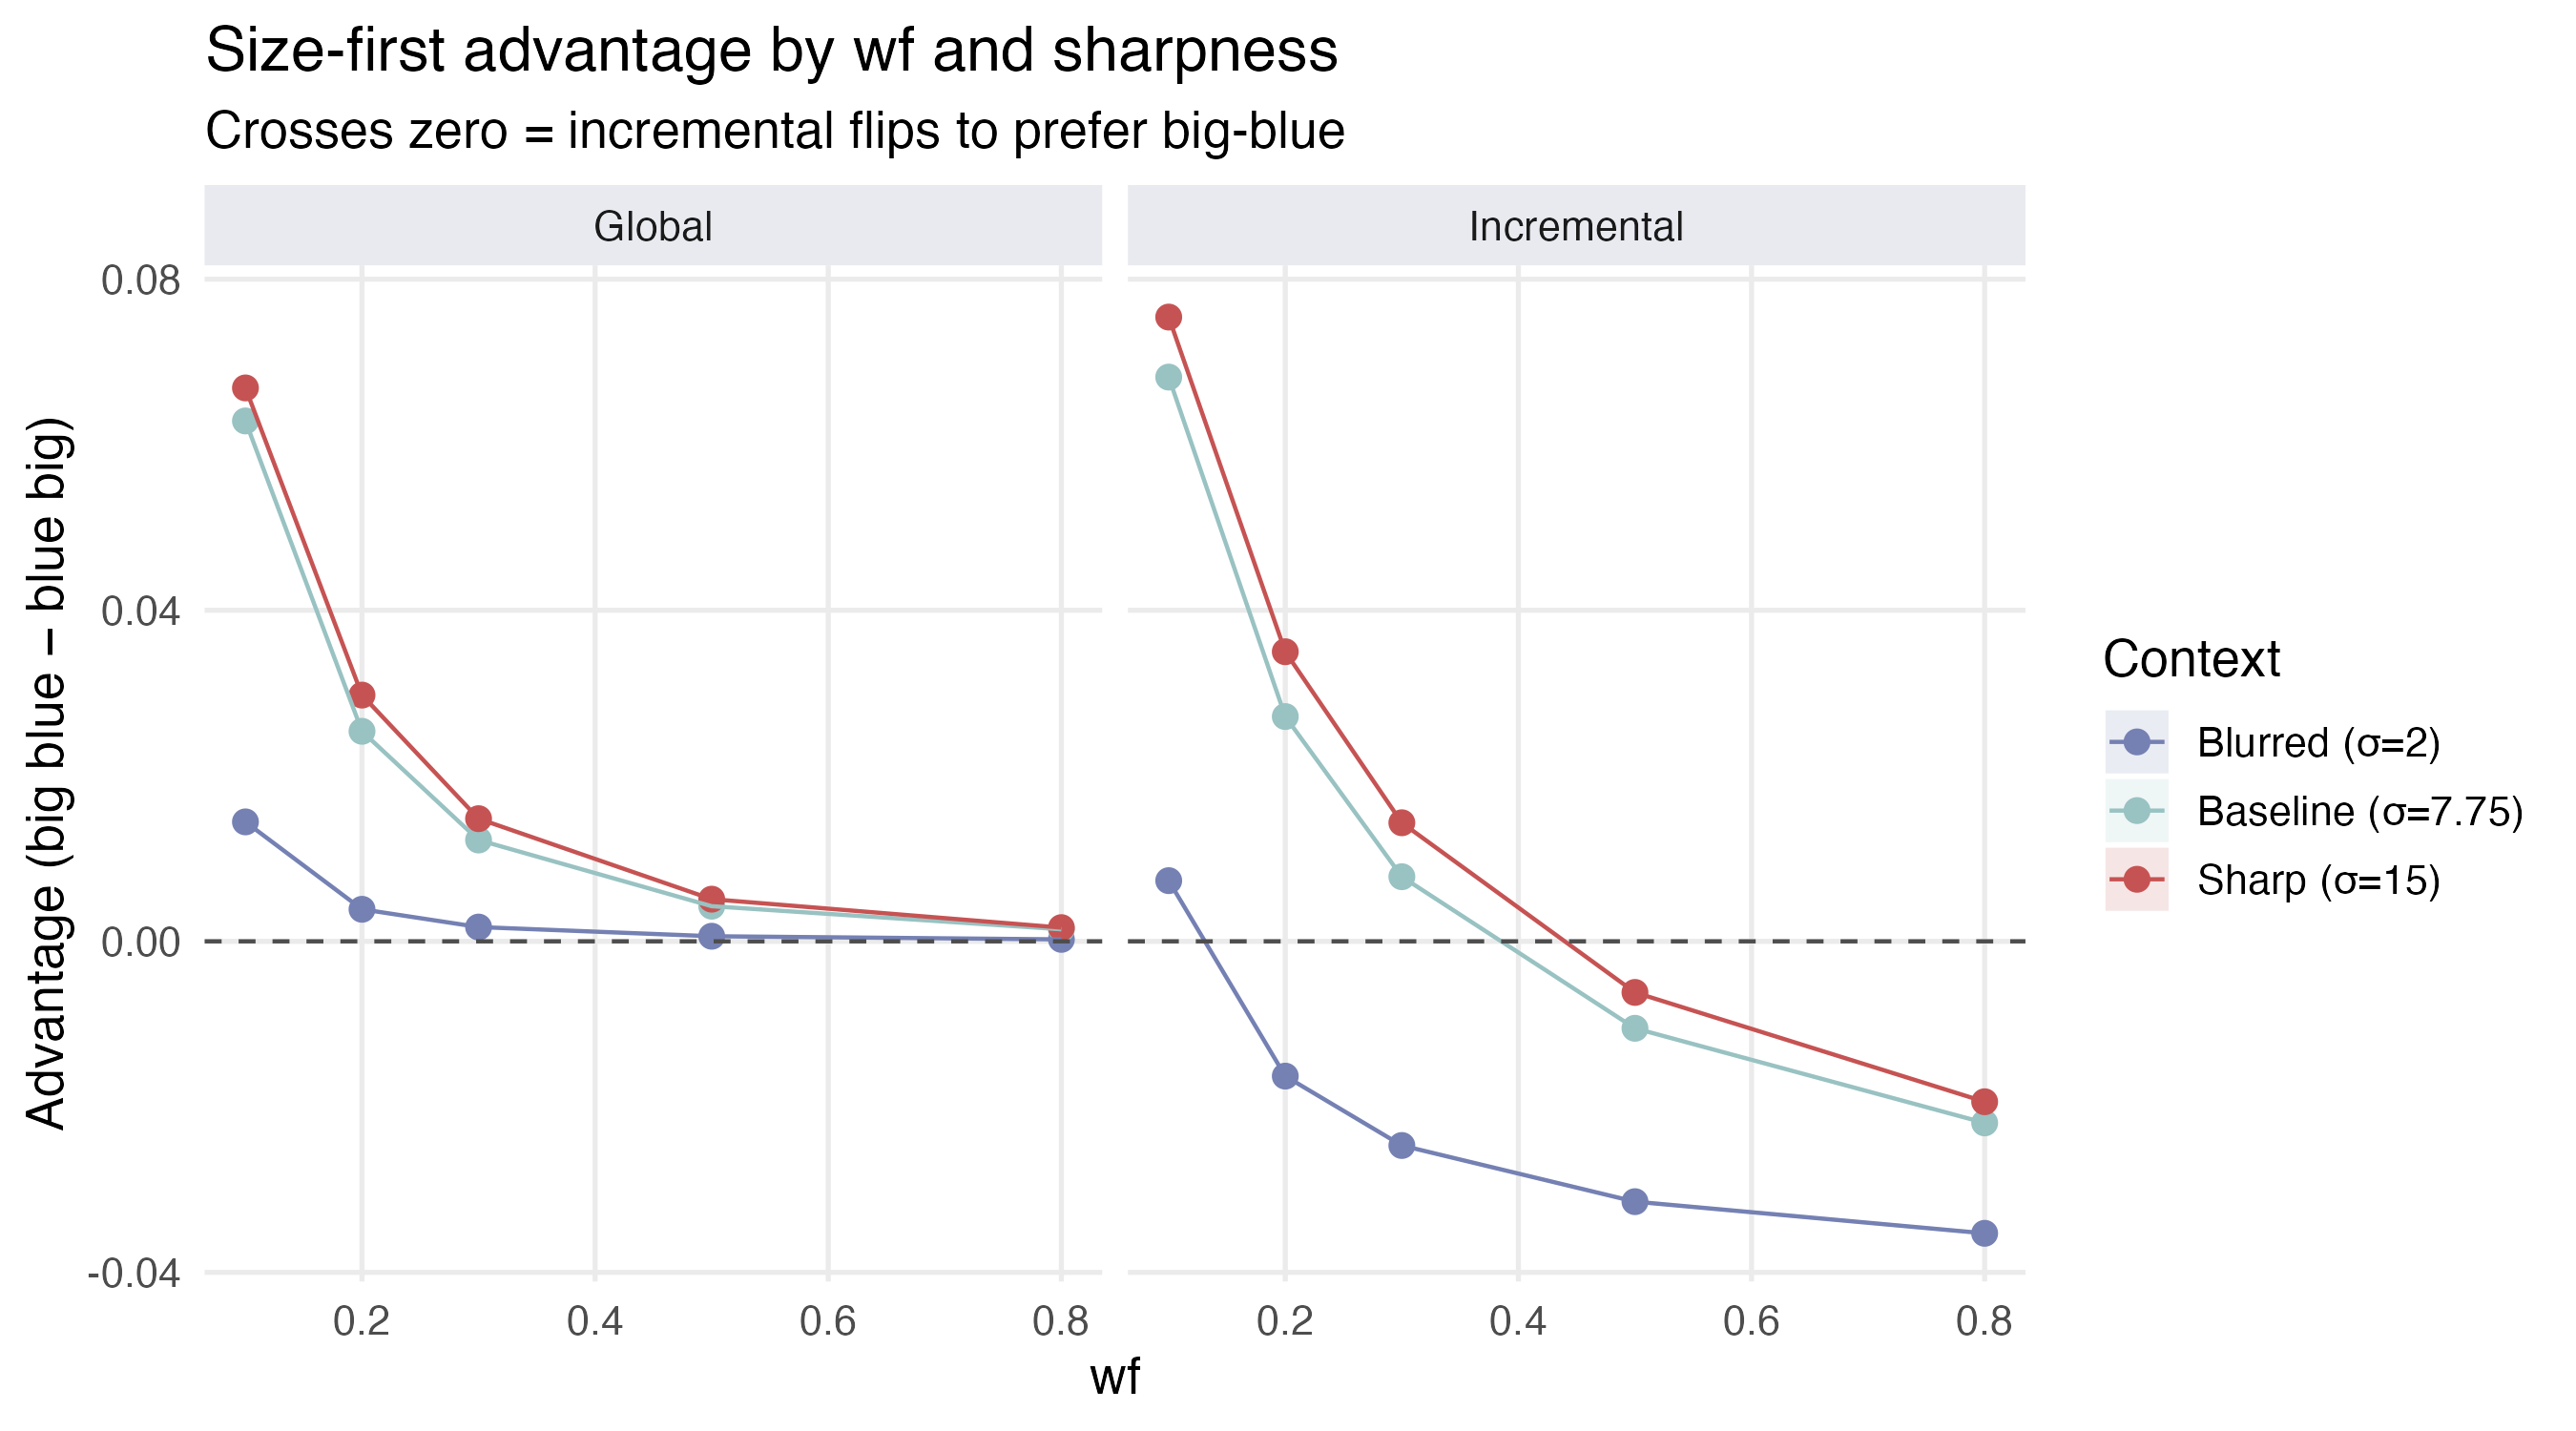
\includegraphics[width=\columnwidth]{../04-simulation-w-randomstates/sim_advantage_wf_sd.png}
  \caption{Mean size-first advantage ($\Delta$) as a function of perceptual
    blur $\omega$ for incremental and global speakers under recursive
    semantics, broken down by context sharpness $\sigma_{\text{sd}}$.
    Error bands show $\pm 2$ SE.
    The dashed line marks $\Delta = 0$.
    The global speaker is insensitive to $\omega$; the incremental speaker
    crosses from negative to positive at $\omega \approx 0.30$.}
  \label{fig:adv-wf}
\end{figure}

Table~\ref{tab:wf-sd} reports mean $\Delta$ at each combination of
$\omega$ and $\sigma_{\text{sd}}$ for the incremental speaker under
recursive semantics.
At $\omega = 0.1$, sharp contexts ($\sigma_{\text{sd}} = 15$) produce
$\Delta = +0.074$, approximately five times the global-speaker advantage,
while blurred contexts ($\sigma_{\text{sd}} = 2$) yield only $+0.006$.
This interaction occurs because a sharp context distributes objects
across a wide size range, making the size adjective highly diagnostic
when $\omega$ is small.
In a blurred context, objects cluster near a common size, and even a
steep CDF cannot make ``big'' much more discriminating than chance.

\begin{table}[h]
\centering
\small
\caption{Mean size-first advantage $\Delta$ for the incremental speaker
  under recursive semantics,
  by perceptual blur $\omega$ and context sharpness $\sigma_{\text{sd}}$.}
\label{tab:wf-sd}
\begin{tabular}{lccc}
\toprule
 & \multicolumn{3}{c}{$\sigma_{\text{sd}}$} \\
\cmidrule(lr){2-4}
$\omega$ & 2.0 & 7.75 & 15.0 \\
\midrule
0.1 & $+0.006$ & $+0.067$ & $+0.074$ \\
0.2 & $-0.017$ & $+0.027$ & $+0.034$ \\
0.3 & $-0.025$ & $+0.007$ & $+0.014$ \\
0.5 & $-0.032$ & $-0.011$ & $-0.005$ \\
0.8 & $-0.036$ & $-0.022$ & $-0.018$ \\
\bottomrule
\end{tabular}
\end{table}

\subsubsection{Static Semantics Eliminates the Global Advantage}

The most striking result of the $2 \times 2$ design is that static
semantics completely eliminates the global speaker's size-first advantage.
Under static semantics, the global speaker produced $\Delta = 0.000$
across all parameter combinations without exception.
This occurs because, when the size threshold is held fixed at the
uniform-prior value, the literal listener produces identical posterior
distributions for \textit{big blue} and \textit{blue big}: both orderings
compose the same semantic values over the same prior, differing only in
application order, which is irrelevant when the threshold does not update.
The global speaker, which selects between complete utterances based on
their literal-listener informativeness, therefore assigns equal probability
to both orderings for every referent.

The incremental speaker under static semantics produced a mean advantage
of $\Delta = -0.009$, with only 33.6\% of parameter combinations favoring
size-first — a stronger color-first bias than under recursive semantics
($\Delta = +0.004$).
Without recursive threshold adaptation, the size adjective is less
diagnostic at step~1, amplifying the chain-rule asymmetry that favors
``blue'' as the opening token.

\subsubsection{Role of the Threshold Parameter $k$}

The threshold parameter $k$ has opposite directional effects on the two
speaker architectures under recursive semantics.
For the incremental speaker, higher $k$ (lower threshold; more objects
qualify as ``big'') degrades size-first advantage — increasing $k$ from
0.1 to 0.9 reduces the mean advantage by approximately 0.019 — because a
permissive threshold weakens the discriminating power of ``big.''
For the global speaker, the same manipulation leaves the advantage
virtually unchanged.
Under static semantics, $k$ has no effect on the global speaker (the
advantage is zero everywhere) and amplifies the color-first bias for the
incremental speaker.

\subsubsection{Effect of Context Size}

Figure~\ref{fig:nobj-2x2} shows the size-first advantage as a function
of $n_{\text{obj}}$, faceted by speaker model and semantic regime.
Under recursive semantics (top row), both speakers show their largest
advantages at small $n_{\text{obj}}$, with $\Delta$ converging toward
zero as the context grows and referent probability is diluted across
more objects.
The direction of the advantage is preserved across context sizes for
the global speaker.
For the incremental speaker the direction is parameter-dependent, but
the crossover at $\omega \approx 0.30$ is robust to $n_{\text{obj}}$.

Under static semantics (bottom row), the global speaker shows zero
advantage at all context sizes.
The incremental speaker shows a negative advantage (color-first), most
pronounced at small $n_{\text{obj}}$ with blurred contexts, converging
toward zero as the context grows.

\begin{figure}[h]
  \centering
  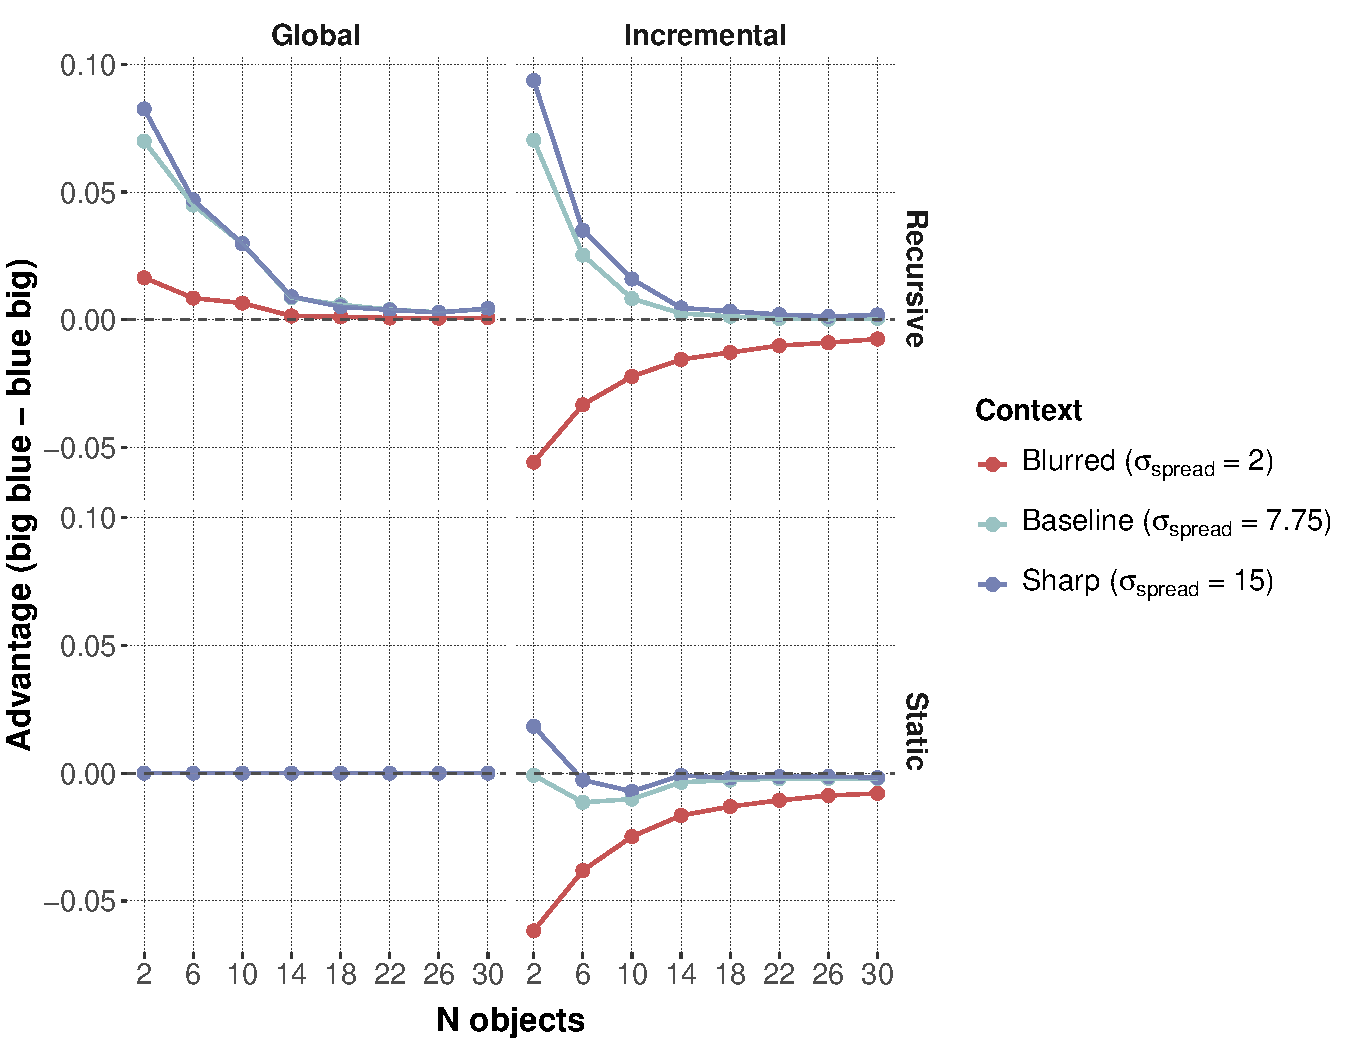
\includegraphics[width=\columnwidth]{figures/sim_advantage_nobj.pdf}
  \caption{Mean size-first advantage ($\Delta$) as a function of context
    size $n_{\text{obj}}$, faceted by speaker model (columns) and semantic
    regime (rows).
    Lines show context sharpness $\sigma_{\text{sd}}$.
    Error bands show $\pm 2$ SE.
    Under static semantics the global speaker produces zero advantage at
    all context sizes; the incremental speaker shows a negative (color-first)
    bias that diminishes with context size.}
  \label{fig:nobj-2x2}
\end{figure}

\subsection{Summary}

The $2 \times 2$ simulation reveals that both speaker architecture and
semantic regime are necessary to predict canonical adjective ordering.
Recursive semantics is required for the global speaker to produce any
size-first advantage at all: under static semantics the two orderings
are informationally equivalent.
The incremental speaker can produce a size-first advantage under
recursive semantics when perceptual blur is low
($\omega \lesssim 0.30$) and context sharpness is high, but defaults
to color-first under static semantics across most of the parameter space.
The critical interaction is between semantic regime and speaker
architecture: recursive semantics creates an asymmetry in the literal
listener that the global speaker exploits directly and that the
incremental speaker can leverage when size is sufficiently diagnostic
at step~1.
These results motivate estimating $\omega$ from empirical
adjective-ordering data rather than fixing it a priori, and they
highlight recursive semantics as a key architectural choice whose
contribution can be isolated from the speaker's composition strategy.

% =============================================================================

\section{Simulation}

\subsection{Overview}

A factorial simulation examined how two RSA speaker architectures and two
semantic regimes jointly determine the size-first advantage.
The speaker factor crosses an \textit{incremental} speaker that composes
utterances token-by-token via a chain rule with a \textit{global} speaker
that evaluates full two-word utterances at once.
The semantics factor crosses \textit{recursive} semantics, in which the
size threshold adapts to the listener's running posterior at each
composition step, with \textit{static} semantics, in which the threshold is
computed once from the uniform prior and held fixed.
The central measure is communicative success: the probability that a
pragmatic listener, reasoning about the speaker, recovers the intended
referent from a given utterance.
Size-first (\textit{big blue}) is taken to be preferred whenever it yields
strictly higher communicative success than color-first (\textit{blue big}).

\subsection{Model}

\paragraph{Referents and contexts.}
Each context consists of $n_{\text{obj}}$ objects drawn from a
log-normal size distribution with spread parameter $\sigma_{\text{sd}}$,
with each draw independently assigned a uniformly random color (0 or 1) and
form (0 or 1).
The intended referent is always the object with the largest size, color
$= 1$ (``blue''), and form $= 1$.
The uniform object prior is $P(s) = 1/n_{\text{obj}}$.

\paragraph{Adjective semantics.}
For a color adjective (``blue''),
\begin{equation}
  \llbracket \text{blue} \rrbracket(s) \;=\;
  c_s \cdot v_c + (1 - c_s)(1 - v_c),
\end{equation}
where $c_s \in \{0,1\}$ is the object's color feature and
$v_c \in (0.5, 1)$ is the color semantic value (how reliably the word
maps to the feature).

For a size adjective (``big''), applicability is modeled as a
cumulative-normal threshold function with perceptual blur $\omega$:
\begin{equation}
  \llbracket \text{big} \rrbracket(s) \;=\;
  \Phi\!\left(\frac{s - \theta}{\omega\sqrt{s^2 + \theta^2}}\right),
\end{equation}
where $\theta$ is a context-sensitive threshold and
$\omega$ controls sharpness: small $\omega$ produces a steep CDF
so that only the very largest object receives high applicability.

\paragraph{Threshold.}
The threshold $\theta$ is defined over the mid-range of the context
distribution $C$,
\begin{equation}
  \theta_k(C) \;=\;
  x_{\max}^{\text{mid}}(C) - k\bigl(x_{\max}^{\text{mid}}(C) - x_{\min}^{\text{mid}}(C)\bigr),
\end{equation}
where $x_{\min}^{\text{mid}}$ and $x_{\max}^{\text{mid}}$ are the
20th- and 80th-percentile sizes in $C$, and $k \in [0,1]$ shifts
the threshold between the top and the middle of the mid-range.
Higher $k$ lowers the threshold, admitting more objects as ``big.''

\paragraph{Literal listener.}
For single-word utterances,
$L_0(s \mid w) \propto \llbracket w \rrbracket(s) \cdot P(s)$.
For two-word utterances $u = w_1 w_2$, the literal listener applies
backward functional composition, processing tokens right-to-left and
updating the posterior at each step.
Under \textit{recursive} semantics, the size threshold $\theta$ is
recomputed from this running posterior before each token is applied, so the
threshold adapts to the listener's evolving belief state.
Under \textit{static} semantics, $\theta$ is computed once from the uniform
prior and held fixed throughout composition.
In both cases the final result is
$L_0(s \mid w_1 w_2) \propto
  \llbracket w_1 \rrbracket(s) \cdot \llbracket w_2 \rrbracket(s) \cdot P(s)$,
but under recursive semantics the semantic values of the size adjective
differ between the two orderings because the threshold depends on which
token was processed first.

\paragraph{Global speaker.}
The global speaker evaluates both full two-word utterances simultaneously,
\begin{equation}
  S_G(u \mid s) \;\propto\; \bigl[L_0(s \mid u)\bigr]^\alpha,
  \quad u \in \{\text{big-blue},\; \text{blue-big}\},
\end{equation}
treating each ordering as an atomic unit.

\paragraph{Incremental speaker.}
The incremental speaker applies a two-step chain rule
following \citeA{cohn-gordon-et-al2019}.
At step 1, it selects a first token by reasoning over the single-word
literal listener:
\begin{equation}
  S_1(w_1 \mid s)
    \;\propto\; \bigl[L_0(s \mid w_1)\bigr]^\alpha.
\end{equation}
At step 2, given prefix $w_1$, it decides whether to continue:
\begin{equation}
  S_2(w_2 \mid w_1, s)
    \;\propto\; \bigl[L_0(s \mid w_1 w_2)\bigr]^\alpha,
\end{equation}
where the alternative is stopping at the single word $w_1$.
The full utterance probability is then
\begin{equation}
  S_I(w_1 w_2 \mid s) \;=\; S_1(w_1 \mid s) \cdot S_2(w_2 \mid w_1, s).
  \label{eq:inc-chain}
\end{equation}

\paragraph{Pragmatic listener.}
The pragmatic listener inverts the speaker distribution via Bayes' rule
with a uniform prior over referents,
\begin{equation}
  L_1(s \mid u) \;\propto\; S(u \mid s) \cdot P(s).
\end{equation}
The primary dependent variable is the \textit{size-first advantage},
\begin{equation}
  \Delta(s) \;=\;
  L_1(s^* \mid \text{big-blue}) - L_1(s^* \mid \text{blue-big}),
\end{equation}
where $s^*$ is the intended referent.
Positive values indicate that the size-first order yields higher
communicative success.

\subsection{Parameter Sweep}

Seven parameters were varied factorially (Table~\ref{tab:params}).
For each combination, 1{,}000 contexts were sampled, yielding
12{,}000{,}000 rows total.
The simulation was implemented in JAX \citep{jax2018github} and executed
in a single vectorized pass using nested \texttt{vmap}/\texttt{jit},
completing in under 90 seconds on CPU.

\begin{table}[h]
\centering
\small
\caption{Simulation parameter grid.}
\label{tab:params}
\begin{tabular}{llc}
\toprule
Parameter & Values & $n$ \\
\midrule
$n_{\text{obj}}$    & 2, 6, 10, 14, 18, 22, 26, 30 & 8 \\
Speaker model       & incremental, global           & 2 \\
Semantics           & recursive, static             & 2 \\
$v_c$ (color sem.)  & 0.90, 0.92, 0.94, 0.96, 0.98 & 5 \\
$k$ (threshold)     & 0.1, 0.3, 0.5, 0.7, 0.9      & 5 \\
$\omega$ (blur)     & 0.1, 0.2, 0.3, 0.5, 0.8      & 5 \\
$\sigma_{\text{sd}}$ (context spread) & 2.0, 7.75, 15.0 & 3 \\
\midrule
\multicolumn{2}{l}{Fixed: $\alpha = 1$, bias $= 0$, utterance length $= 2$} & \\
\bottomrule
\end{tabular}
\end{table}

\subsection{Results}

\subsubsection{Recursive Semantics: Global Speaker}

Under recursive semantics, the global speaker produced a consistent
size-first advantage across virtually all parameter combinations.
Averaging over all contexts and parameter values, it assigned
$L_1(s^* \mid \text{big-blue}) = 0.138$ versus
$L_1(s^* \mid \text{blue-big}) = 0.122$,
yielding a mean advantage of $\Delta = +0.016$.
Across individual parameter combinations, 64.8\% produced a positive
advantage, and the direction was preserved across all levels of
$n_{\text{obj}}$, $\sigma_{\text{sd}}$, and $v_c$.

The preference arises because, under recursive semantics, the size
threshold shifts when ``big'' versus ``blue'' is processed first.
This asymmetry in the literal listener makes the two orderings
non-equivalent, and the global speaker exploits the ordering that
maximizes referent recovery.

\subsubsection{Recursive Semantics: Incremental Speaker}

Under recursive semantics, the incremental speaker showed a qualitatively
different pattern depending on the perceptual blur parameter $\omega$.
At $\omega = 0.5$ (the default in prior work), the incremental speaker
produced a \textit{negative} mean advantage ($\Delta = -0.016$),
with only 23.7\% of parameter combinations favoring size-first.
This reversal reflects a structural asymmetry in the chain rule
(Equation~\ref{eq:inc-chain}):
The referent is by construction the only object with color $= 1$, so
$\llbracket \text{blue} \rrbracket(s^*)$ is close to $v_c$ ($\approx 0.90$--$0.98$)
while $\llbracket \text{blue} \rrbracket(s)$ for any non-referent is close to
$1 - v_c$ ($\approx 0.02$--$0.10$).
The color adjective thus almost perfectly identifies the referent at
step~1.
The size adjective, however, depends on $\omega$: at large $\omega$,
the CDF is shallow and multiple objects receive moderate size
applicability, reducing the discriminating power of ``big'' relative to
``blue.''
When ``blue'' is the more informative first token, the incremental
speaker prefers to say it first, producing \textit{blue big}.

Reducing $\omega$ sharpens the size CDF so that only the largest object
receives high applicability, restoring size as a reliable discriminator at
step~1.
Figure~\ref{fig:adv-wf} shows a monotone relationship between $\omega$
and $\Delta$ for the incremental speaker: the size-first advantage crosses
zero at approximately $\omega \approx 0.30$, and reaches a mean of
$+0.049$ at $\omega = 0.1$.

\begin{figure}[h]
  \centering
  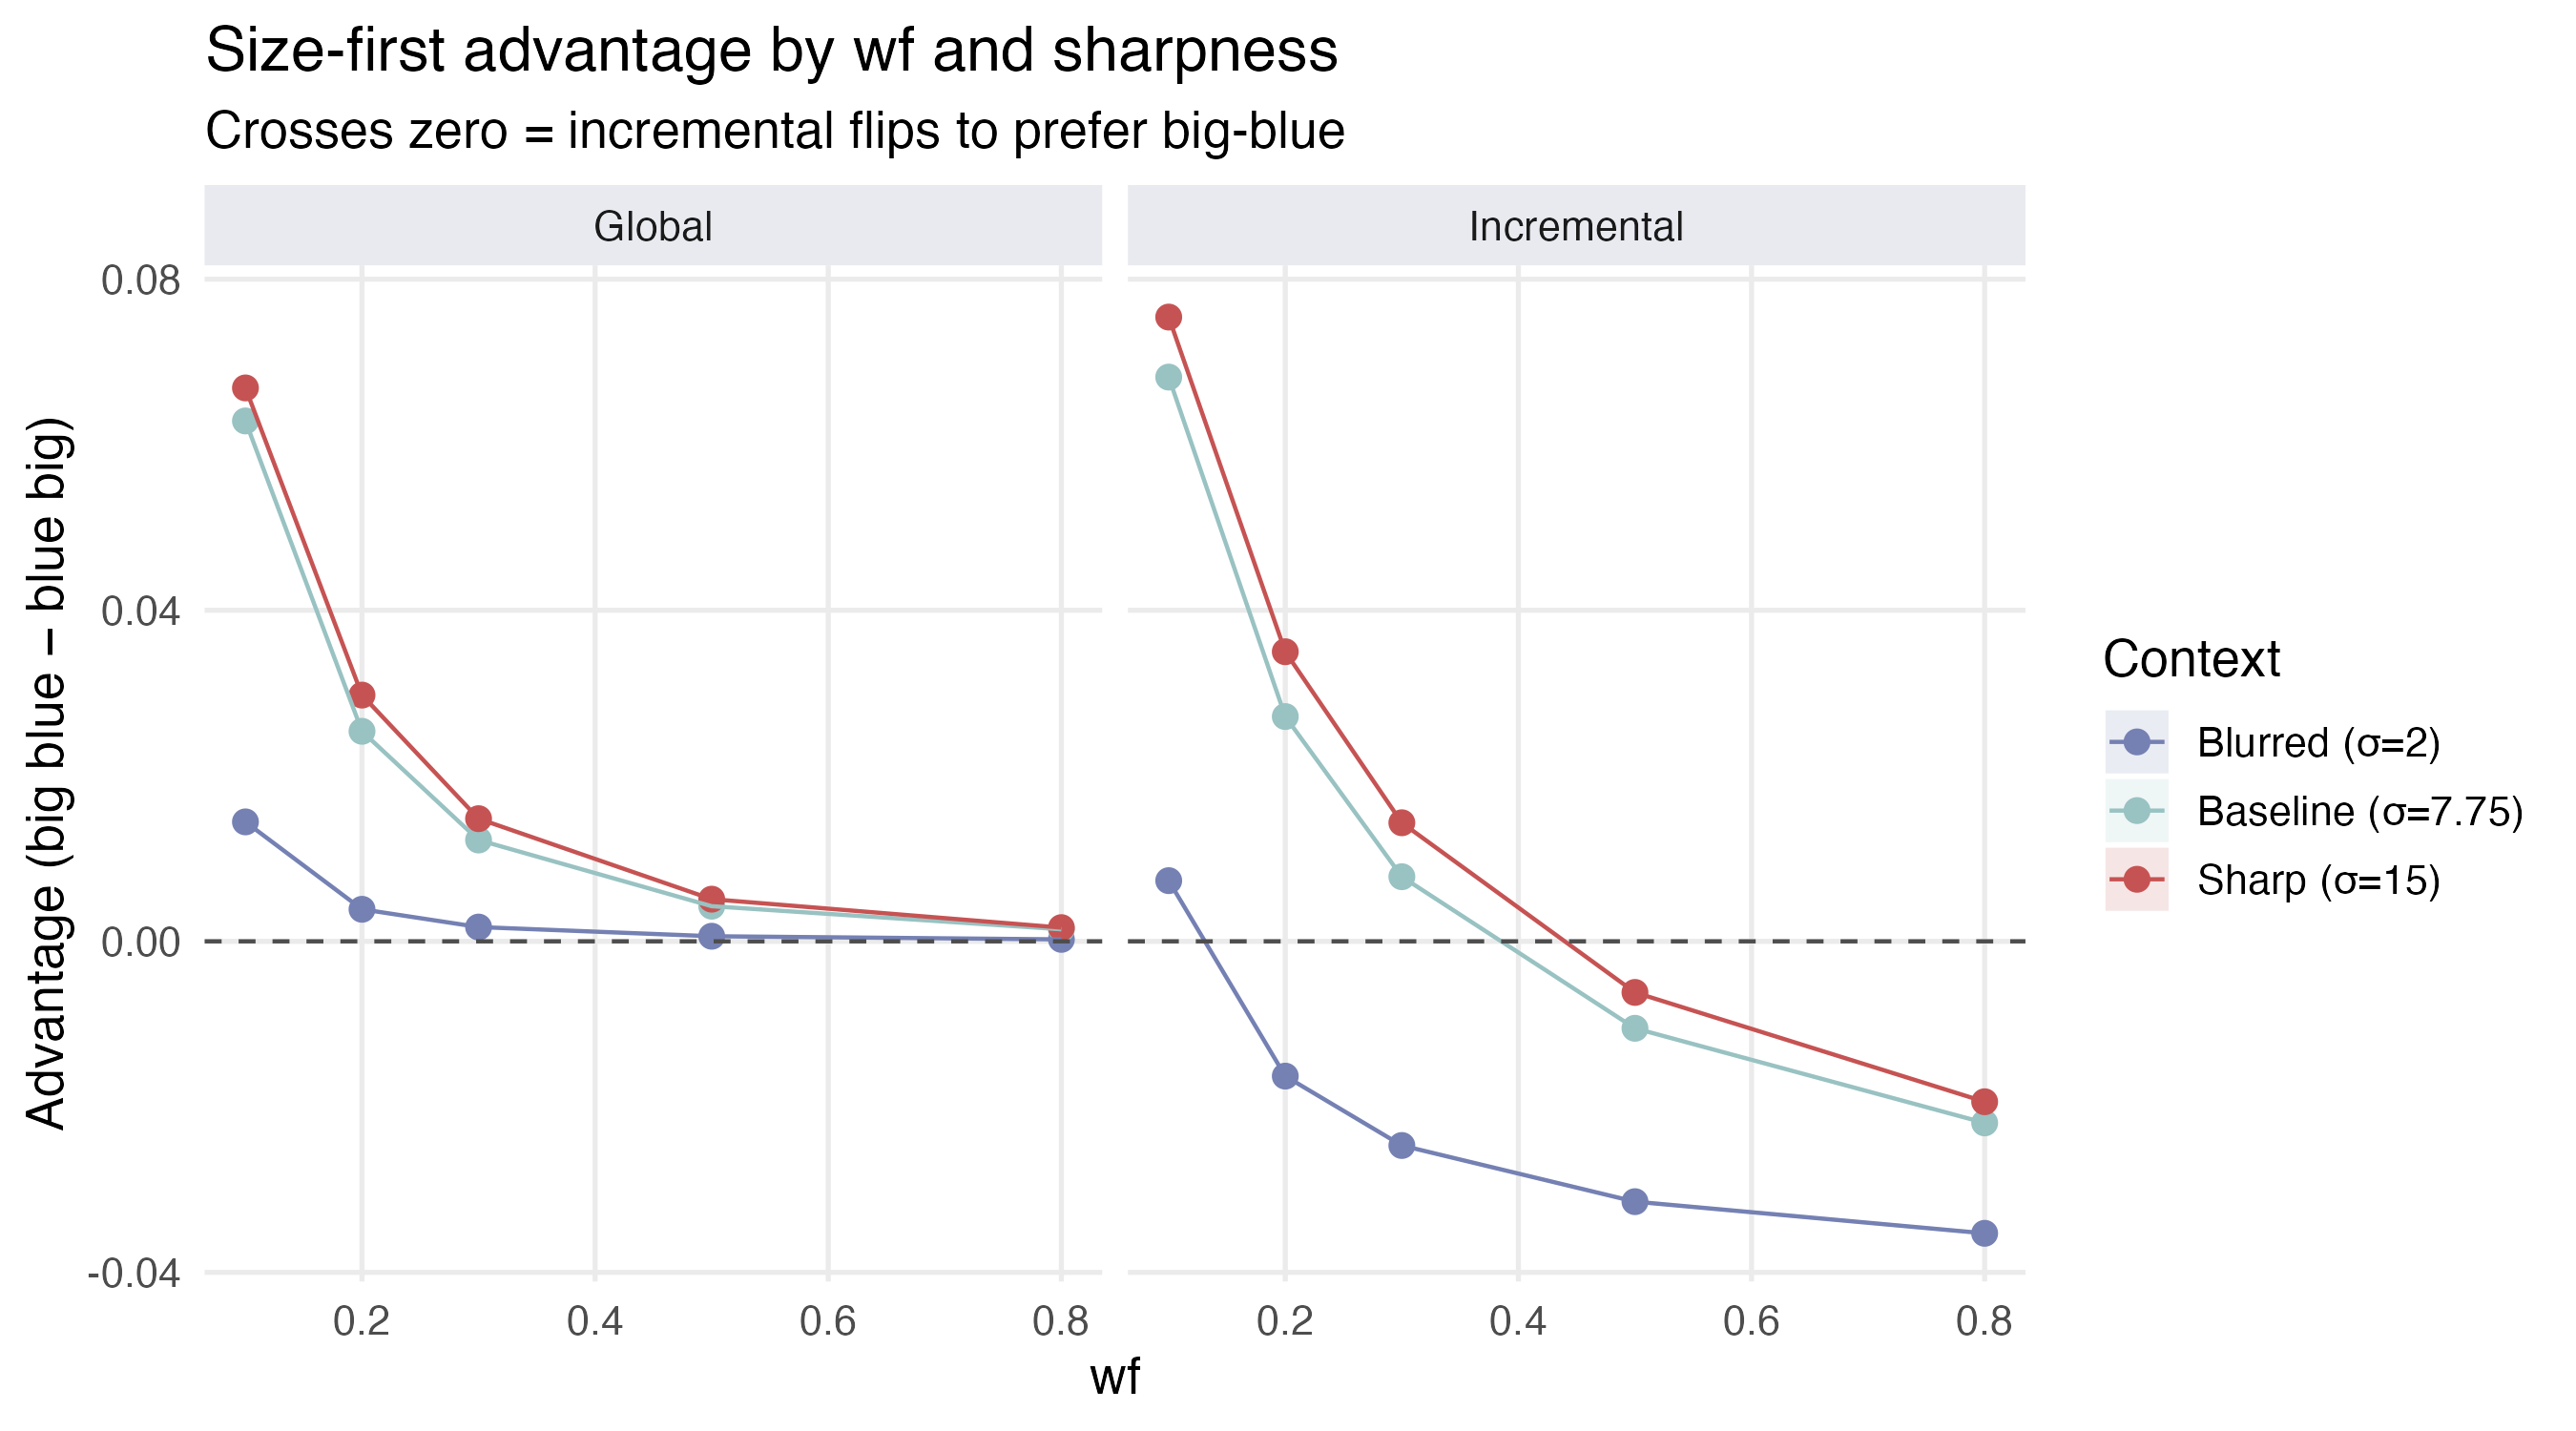
\includegraphics[width=\columnwidth]{../04-simulation-w-randomstates/sim_advantage_wf_sd.png}
  \caption{Mean size-first advantage ($\Delta$) as a function of perceptual
    blur $\omega$ for incremental and global speakers under recursive
    semantics, broken down by context sharpness $\sigma_{\text{sd}}$.
    Error bands show $\pm 2$ SE.
    The dashed line marks $\Delta = 0$.
    The global speaker is insensitive to $\omega$; the incremental speaker
    crosses from negative to positive at $\omega \approx 0.30$.}
  \label{fig:adv-wf}
\end{figure}

Table~\ref{tab:wf-sd} reports mean $\Delta$ at each combination of
$\omega$ and $\sigma_{\text{sd}}$ for the incremental speaker under
recursive semantics.
At $\omega = 0.1$, sharp contexts ($\sigma_{\text{sd}} = 15$) produce
$\Delta = +0.074$, approximately five times the global-speaker advantage,
while blurred contexts ($\sigma_{\text{sd}} = 2$) yield only $+0.006$.
This interaction occurs because a sharp context distributes objects
across a wide size range, making the size adjective highly diagnostic
when $\omega$ is small.
In a blurred context, objects cluster near a common size, and even a
steep CDF cannot make ``big'' much more discriminating than chance.

\begin{table}[h]
\centering
\small
\caption{Mean size-first advantage $\Delta$ for the incremental speaker
  under recursive semantics,
  by perceptual blur $\omega$ and context sharpness $\sigma_{\text{sd}}$.}
\label{tab:wf-sd}
\begin{tabular}{lccc}
\toprule
 & \multicolumn{3}{c}{$\sigma_{\text{sd}}$} \\
\cmidrule(lr){2-4}
$\omega$ & 2.0 & 7.75 & 15.0 \\
\midrule
0.1 & $+0.006$ & $+0.067$ & $+0.074$ \\
0.2 & $-0.017$ & $+0.027$ & $+0.034$ \\
0.3 & $-0.025$ & $+0.007$ & $+0.014$ \\
0.5 & $-0.032$ & $-0.011$ & $-0.005$ \\
0.8 & $-0.036$ & $-0.022$ & $-0.018$ \\
\bottomrule
\end{tabular}
\end{table}

\subsubsection{Static Semantics Eliminates the Global Advantage}

The most striking result of the $2 \times 2$ design is that static
semantics completely eliminates the global speaker's size-first advantage.
Under static semantics, the global speaker produced $\Delta = 0.000$
across all parameter combinations without exception.
This occurs because, when the size threshold is held fixed at the
uniform-prior value, the literal listener produces identical posterior
distributions for \textit{big blue} and \textit{blue big}: both orderings
compose the same semantic values over the same prior, differing only in
application order, which is irrelevant when the threshold does not update.
The global speaker, which selects between complete utterances based on
their literal-listener informativeness, therefore assigns equal probability
to both orderings for every referent.

The incremental speaker under static semantics produced a mean advantage
of $\Delta = -0.009$, with only 33.6\% of parameter combinations favoring
size-first — a stronger color-first bias than under recursive semantics
($\Delta = +0.004$).
Without recursive threshold adaptation, the size adjective is less
diagnostic at step~1, amplifying the chain-rule asymmetry that favors
``blue'' as the opening token.

\subsubsection{Role of the Threshold Parameter $k$}

The threshold parameter $k$ has opposite directional effects on the two
speaker architectures under recursive semantics.
For the incremental speaker, higher $k$ (lower threshold; more objects
qualify as ``big'') degrades size-first advantage — increasing $k$ from
0.1 to 0.9 reduces the mean advantage by approximately 0.019 — because a
permissive threshold weakens the discriminating power of ``big.''
For the global speaker, the same manipulation leaves the advantage
virtually unchanged.
Under static semantics, $k$ has no effect on the global speaker (the
advantage is zero everywhere) and amplifies the color-first bias for the
incremental speaker.

\subsubsection{Effect of Context Size}

Figure~\ref{fig:nobj-2x2} shows the size-first advantage as a function
of $n_{\text{obj}}$, faceted by speaker model and semantic regime.
Under recursive semantics (top row), both speakers show their largest
advantages at small $n_{\text{obj}}$, with $\Delta$ converging toward
zero as the context grows and referent probability is diluted across
more objects.
The direction of the advantage is preserved across context sizes for
the global speaker.
For the incremental speaker the direction is parameter-dependent, but
the crossover at $\omega \approx 0.30$ is robust to $n_{\text{obj}}$.

Under static semantics (bottom row), the global speaker shows zero
advantage at all context sizes.
The incremental speaker shows a negative advantage (color-first), most
pronounced at small $n_{\text{obj}}$ with blurred contexts, converging
toward zero as the context grows.

\begin{figure}[h]
  \centering
  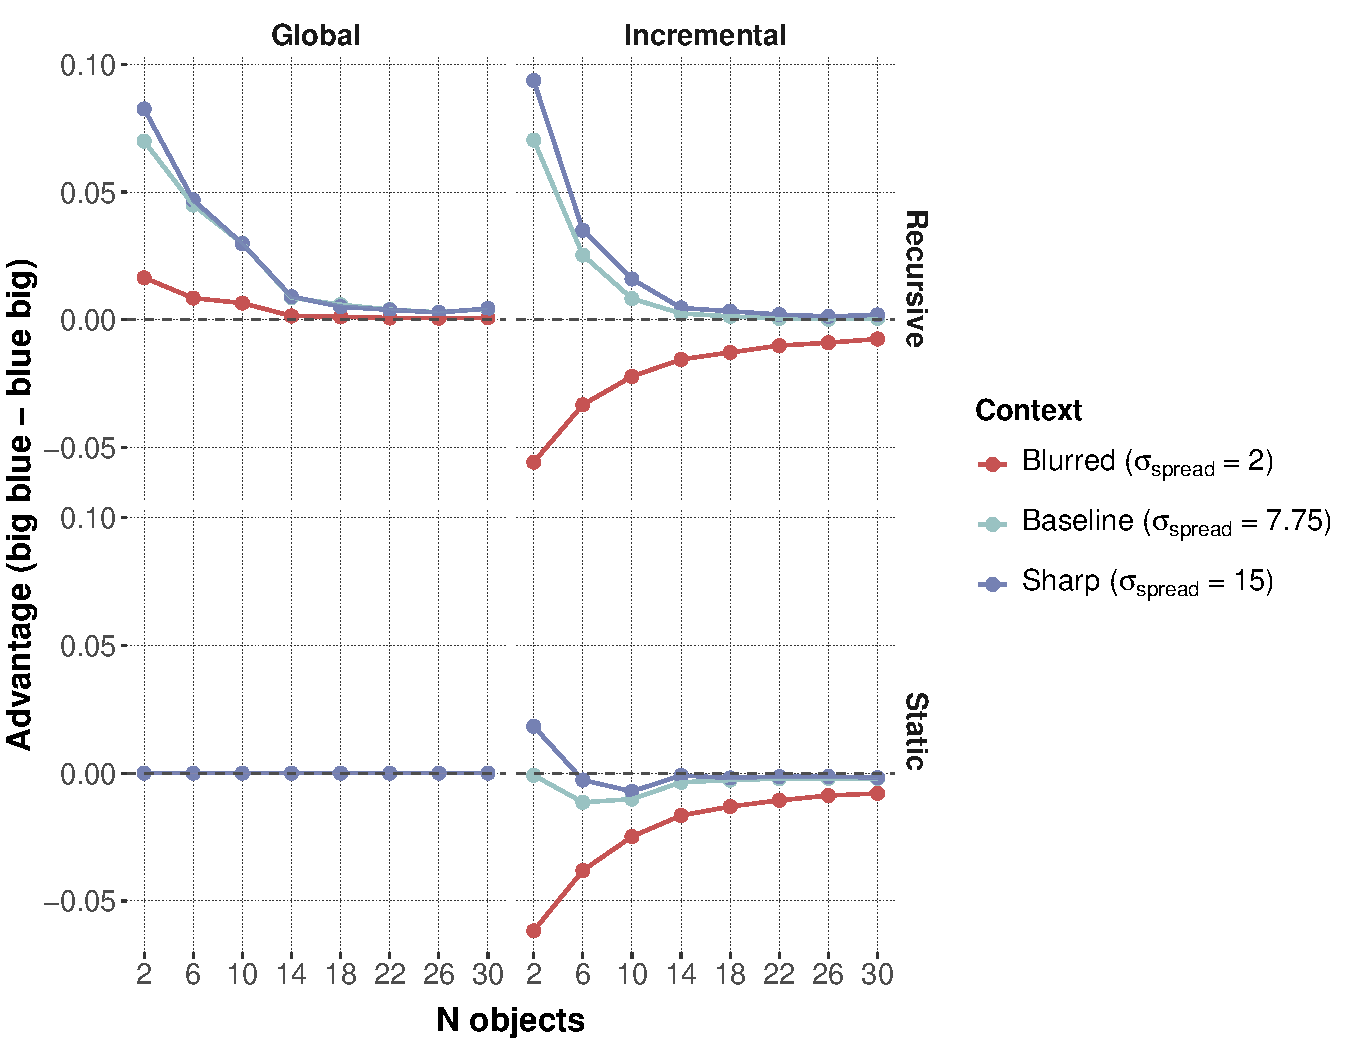
\includegraphics[width=\columnwidth]{figures/sim_advantage_nobj.pdf}
  \caption{Mean size-first advantage ($\Delta$) as a function of context
    size $n_{\text{obj}}$, faceted by speaker model (columns) and semantic
    regime (rows).
    Lines show context sharpness $\sigma_{\text{sd}}$.
    Error bands show $\pm 2$ SE.
    Under static semantics the global speaker produces zero advantage at
    all context sizes; the incremental speaker shows a negative (color-first)
    bias that diminishes with context size.}
  \label{fig:nobj-2x2}
\end{figure}

\subsection{Summary}

The $2 \times 2$ simulation reveals that both speaker architecture and
semantic regime are necessary to predict canonical adjective ordering.
Recursive semantics is required for the global speaker to produce any
size-first advantage at all: under static semantics the two orderings
are informationally equivalent.
The incremental speaker can produce a size-first advantage under
recursive semantics when perceptual blur is low
($\omega \lesssim 0.30$) and context sharpness is high, but defaults
to color-first under static semantics across most of the parameter space.
The critical interaction is between semantic regime and speaker
architecture: recursive semantics creates an asymmetry in the literal
listener that the global speaker exploits directly and that the
incremental speaker can leverage when size is sufficiently diagnostic
at step~1.
These results motivate estimating $\omega$ from empirical
adjective-ordering data rather than fixing it a priori, and they
highlight recursive semantics as a key architectural choice whose
contribution can be isolated from the speaker's composition strategy.

% =============================================================================

\section{Simulation}

\subsection{Overview}

A factorial simulation examined how two RSA speaker architectures and two
semantic regimes jointly determine the size-first advantage.
The speaker factor crosses an \textit{incremental} speaker that composes
utterances token-by-token via a chain rule with a \textit{global} speaker
that evaluates full two-word utterances at once.
The semantics factor crosses \textit{recursive} semantics, in which the
size threshold adapts to the listener's running posterior at each
composition step, with \textit{static} semantics, in which the threshold is
computed once from the uniform prior and held fixed.
The central measure is communicative success: the probability that a
pragmatic listener, reasoning about the speaker, recovers the intended
referent from a given utterance.
Size-first (\textit{big blue}) is taken to be preferred whenever it yields
strictly higher communicative success than color-first (\textit{blue big}).

\subsection{Model}

\paragraph{Referents and contexts.}
Each context consists of $n_{\text{obj}}$ objects drawn from a
log-normal size distribution with spread parameter $\sigma_{\text{sd}}$,
with each draw independently assigned a uniformly random color (0 or 1) and
form (0 or 1).
The intended referent is always the object with the largest size, color
$= 1$ (``blue''), and form $= 1$.
The uniform object prior is $P(s) = 1/n_{\text{obj}}$.

\paragraph{Adjective semantics.}
For a color adjective (``blue''),
\begin{equation}
  \llbracket \text{blue} \rrbracket(s) \;=\;
  c_s \cdot v_c + (1 - c_s)(1 - v_c),
\end{equation}
where $c_s \in \{0,1\}$ is the object's color feature and
$v_c \in (0.5, 1)$ is the color semantic value (how reliably the word
maps to the feature).

For a size adjective (``big''), applicability is modeled as a
cumulative-normal threshold function with perceptual blur $\omega$:
\begin{equation}
  \llbracket \text{big} \rrbracket(s) \;=\;
  \Phi\!\left(\frac{s - \theta}{\omega\sqrt{s^2 + \theta^2}}\right),
\end{equation}
where $\theta$ is a context-sensitive threshold and
$\omega$ controls sharpness: small $\omega$ produces a steep CDF
so that only the very largest object receives high applicability.

\paragraph{Threshold.}
The threshold $\theta$ is defined over the mid-range of the context
distribution $C$,
\begin{equation}
  \theta_k(C) \;=\;
  x_{\max}^{\text{mid}}(C) - k\bigl(x_{\max}^{\text{mid}}(C) - x_{\min}^{\text{mid}}(C)\bigr),
\end{equation}
where $x_{\min}^{\text{mid}}$ and $x_{\max}^{\text{mid}}$ are the
20th- and 80th-percentile sizes in $C$, and $k \in [0,1]$ shifts
the threshold between the top and the middle of the mid-range.
Higher $k$ lowers the threshold, admitting more objects as ``big.''

\paragraph{Literal listener.}
For single-word utterances,
$L_0(s \mid w) \propto \llbracket w \rrbracket(s) \cdot P(s)$.
For two-word utterances $u = w_1 w_2$, the literal listener applies
backward functional composition, processing tokens right-to-left and
updating the posterior at each step.
Under \textit{recursive} semantics, the size threshold $\theta$ is
recomputed from this running posterior before each token is applied, so the
threshold adapts to the listener's evolving belief state.
Under \textit{static} semantics, $\theta$ is computed once from the uniform
prior and held fixed throughout composition.
In both cases the final result is
$L_0(s \mid w_1 w_2) \propto
  \llbracket w_1 \rrbracket(s) \cdot \llbracket w_2 \rrbracket(s) \cdot P(s)$,
but under recursive semantics the semantic values of the size adjective
differ between the two orderings because the threshold depends on which
token was processed first.

\paragraph{Global speaker.}
The global speaker evaluates both full two-word utterances simultaneously,
\begin{equation}
  S_G(u \mid s) \;\propto\; \bigl[L_0(s \mid u)\bigr]^\alpha,
  \quad u \in \{\text{big-blue},\; \text{blue-big}\},
\end{equation}
treating each ordering as an atomic unit.

\paragraph{Incremental speaker.}
The incremental speaker applies a two-step chain rule
following \citeA{cohn-gordon-et-al2019}.
At step 1, it selects a first token by reasoning over the single-word
literal listener:
\begin{equation}
  S_1(w_1 \mid s)
    \;\propto\; \bigl[L_0(s \mid w_1)\bigr]^\alpha.
\end{equation}
At step 2, given prefix $w_1$, it decides whether to continue:
\begin{equation}
  S_2(w_2 \mid w_1, s)
    \;\propto\; \bigl[L_0(s \mid w_1 w_2)\bigr]^\alpha,
\end{equation}
where the alternative is stopping at the single word $w_1$.
The full utterance probability is then
\begin{equation}
  S_I(w_1 w_2 \mid s) \;=\; S_1(w_1 \mid s) \cdot S_2(w_2 \mid w_1, s).
  \label{eq:inc-chain}
\end{equation}

\paragraph{Pragmatic listener.}
The pragmatic listener inverts the speaker distribution via Bayes' rule
with a uniform prior over referents,
\begin{equation}
  L_1(s \mid u) \;\propto\; S(u \mid s) \cdot P(s).
\end{equation}
The primary dependent variable is the \textit{size-first advantage},
\begin{equation}
  \Delta(s) \;=\;
  L_1(s^* \mid \text{big-blue}) - L_1(s^* \mid \text{blue-big}),
\end{equation}
where $s^*$ is the intended referent.
Positive values indicate that the size-first order yields higher
communicative success.

\subsection{Parameter Sweep}

Seven parameters were varied factorially (Table~\ref{tab:params}).
For each combination, 1{,}000 contexts were sampled, yielding
12{,}000{,}000 rows total.
The simulation was implemented in JAX \citep{jax2018github} and executed
in a single vectorized pass using nested \texttt{vmap}/\texttt{jit},
completing in under 90 seconds on CPU.

\begin{table}[h]
\centering
\small
\caption{Simulation parameter grid.}
\label{tab:params}
\begin{tabular}{llc}
\toprule
Parameter & Values & $n$ \\
\midrule
$n_{\text{obj}}$    & 2, 6, 10, 14, 18, 22, 26, 30 & 8 \\
Speaker model       & incremental, global           & 2 \\
Semantics           & recursive, static             & 2 \\
$v_c$ (color sem.)  & 0.90, 0.92, 0.94, 0.96, 0.98 & 5 \\
$k$ (threshold)     & 0.1, 0.3, 0.5, 0.7, 0.9      & 5 \\
$\omega$ (blur)     & 0.1, 0.2, 0.3, 0.5, 0.8      & 5 \\
$\sigma_{\text{sd}}$ (context spread) & 2.0, 7.75, 15.0 & 3 \\
\midrule
\multicolumn{2}{l}{Fixed: $\alpha = 1$, bias $= 0$, utterance length $= 2$} & \\
\bottomrule
\end{tabular}
\end{table}

\subsection{Results}

\subsubsection{Recursive Semantics: Global Speaker}

Under recursive semantics, the global speaker produced a consistent
size-first advantage across virtually all parameter combinations.
Averaging over all contexts and parameter values, it assigned
$L_1(s^* \mid \text{big-blue}) = 0.138$ versus
$L_1(s^* \mid \text{blue-big}) = 0.122$,
yielding a mean advantage of $\Delta = +0.016$.
Across individual parameter combinations, 64.8\% produced a positive
advantage, and the direction was preserved across all levels of
$n_{\text{obj}}$, $\sigma_{\text{sd}}$, and $v_c$.

The preference arises because, under recursive semantics, the size
threshold shifts when ``big'' versus ``blue'' is processed first.
This asymmetry in the literal listener makes the two orderings
non-equivalent, and the global speaker exploits the ordering that
maximizes referent recovery.

\subsubsection{Recursive Semantics: Incremental Speaker}

Under recursive semantics, the incremental speaker showed a qualitatively
different pattern depending on the perceptual blur parameter $\omega$.
At $\omega = 0.5$ (the default in prior work), the incremental speaker
produced a \textit{negative} mean advantage ($\Delta = -0.016$),
with only 23.7\% of parameter combinations favoring size-first.
This reversal reflects a structural asymmetry in the chain rule
(Equation~\ref{eq:inc-chain}):
The referent is by construction the only object with color $= 1$, so
$\llbracket \text{blue} \rrbracket(s^*)$ is close to $v_c$ ($\approx 0.90$--$0.98$)
while $\llbracket \text{blue} \rrbracket(s)$ for any non-referent is close to
$1 - v_c$ ($\approx 0.02$--$0.10$).
The color adjective thus almost perfectly identifies the referent at
step~1.
The size adjective, however, depends on $\omega$: at large $\omega$,
the CDF is shallow and multiple objects receive moderate size
applicability, reducing the discriminating power of ``big'' relative to
``blue.''
When ``blue'' is the more informative first token, the incremental
speaker prefers to say it first, producing \textit{blue big}.

Reducing $\omega$ sharpens the size CDF so that only the largest object
receives high applicability, restoring size as a reliable discriminator at
step~1.
Figure~\ref{fig:adv-wf} shows a monotone relationship between $\omega$
and $\Delta$ for the incremental speaker: the size-first advantage crosses
zero at approximately $\omega \approx 0.30$, and reaches a mean of
$+0.049$ at $\omega = 0.1$.

\begin{figure}[h]
  \centering
  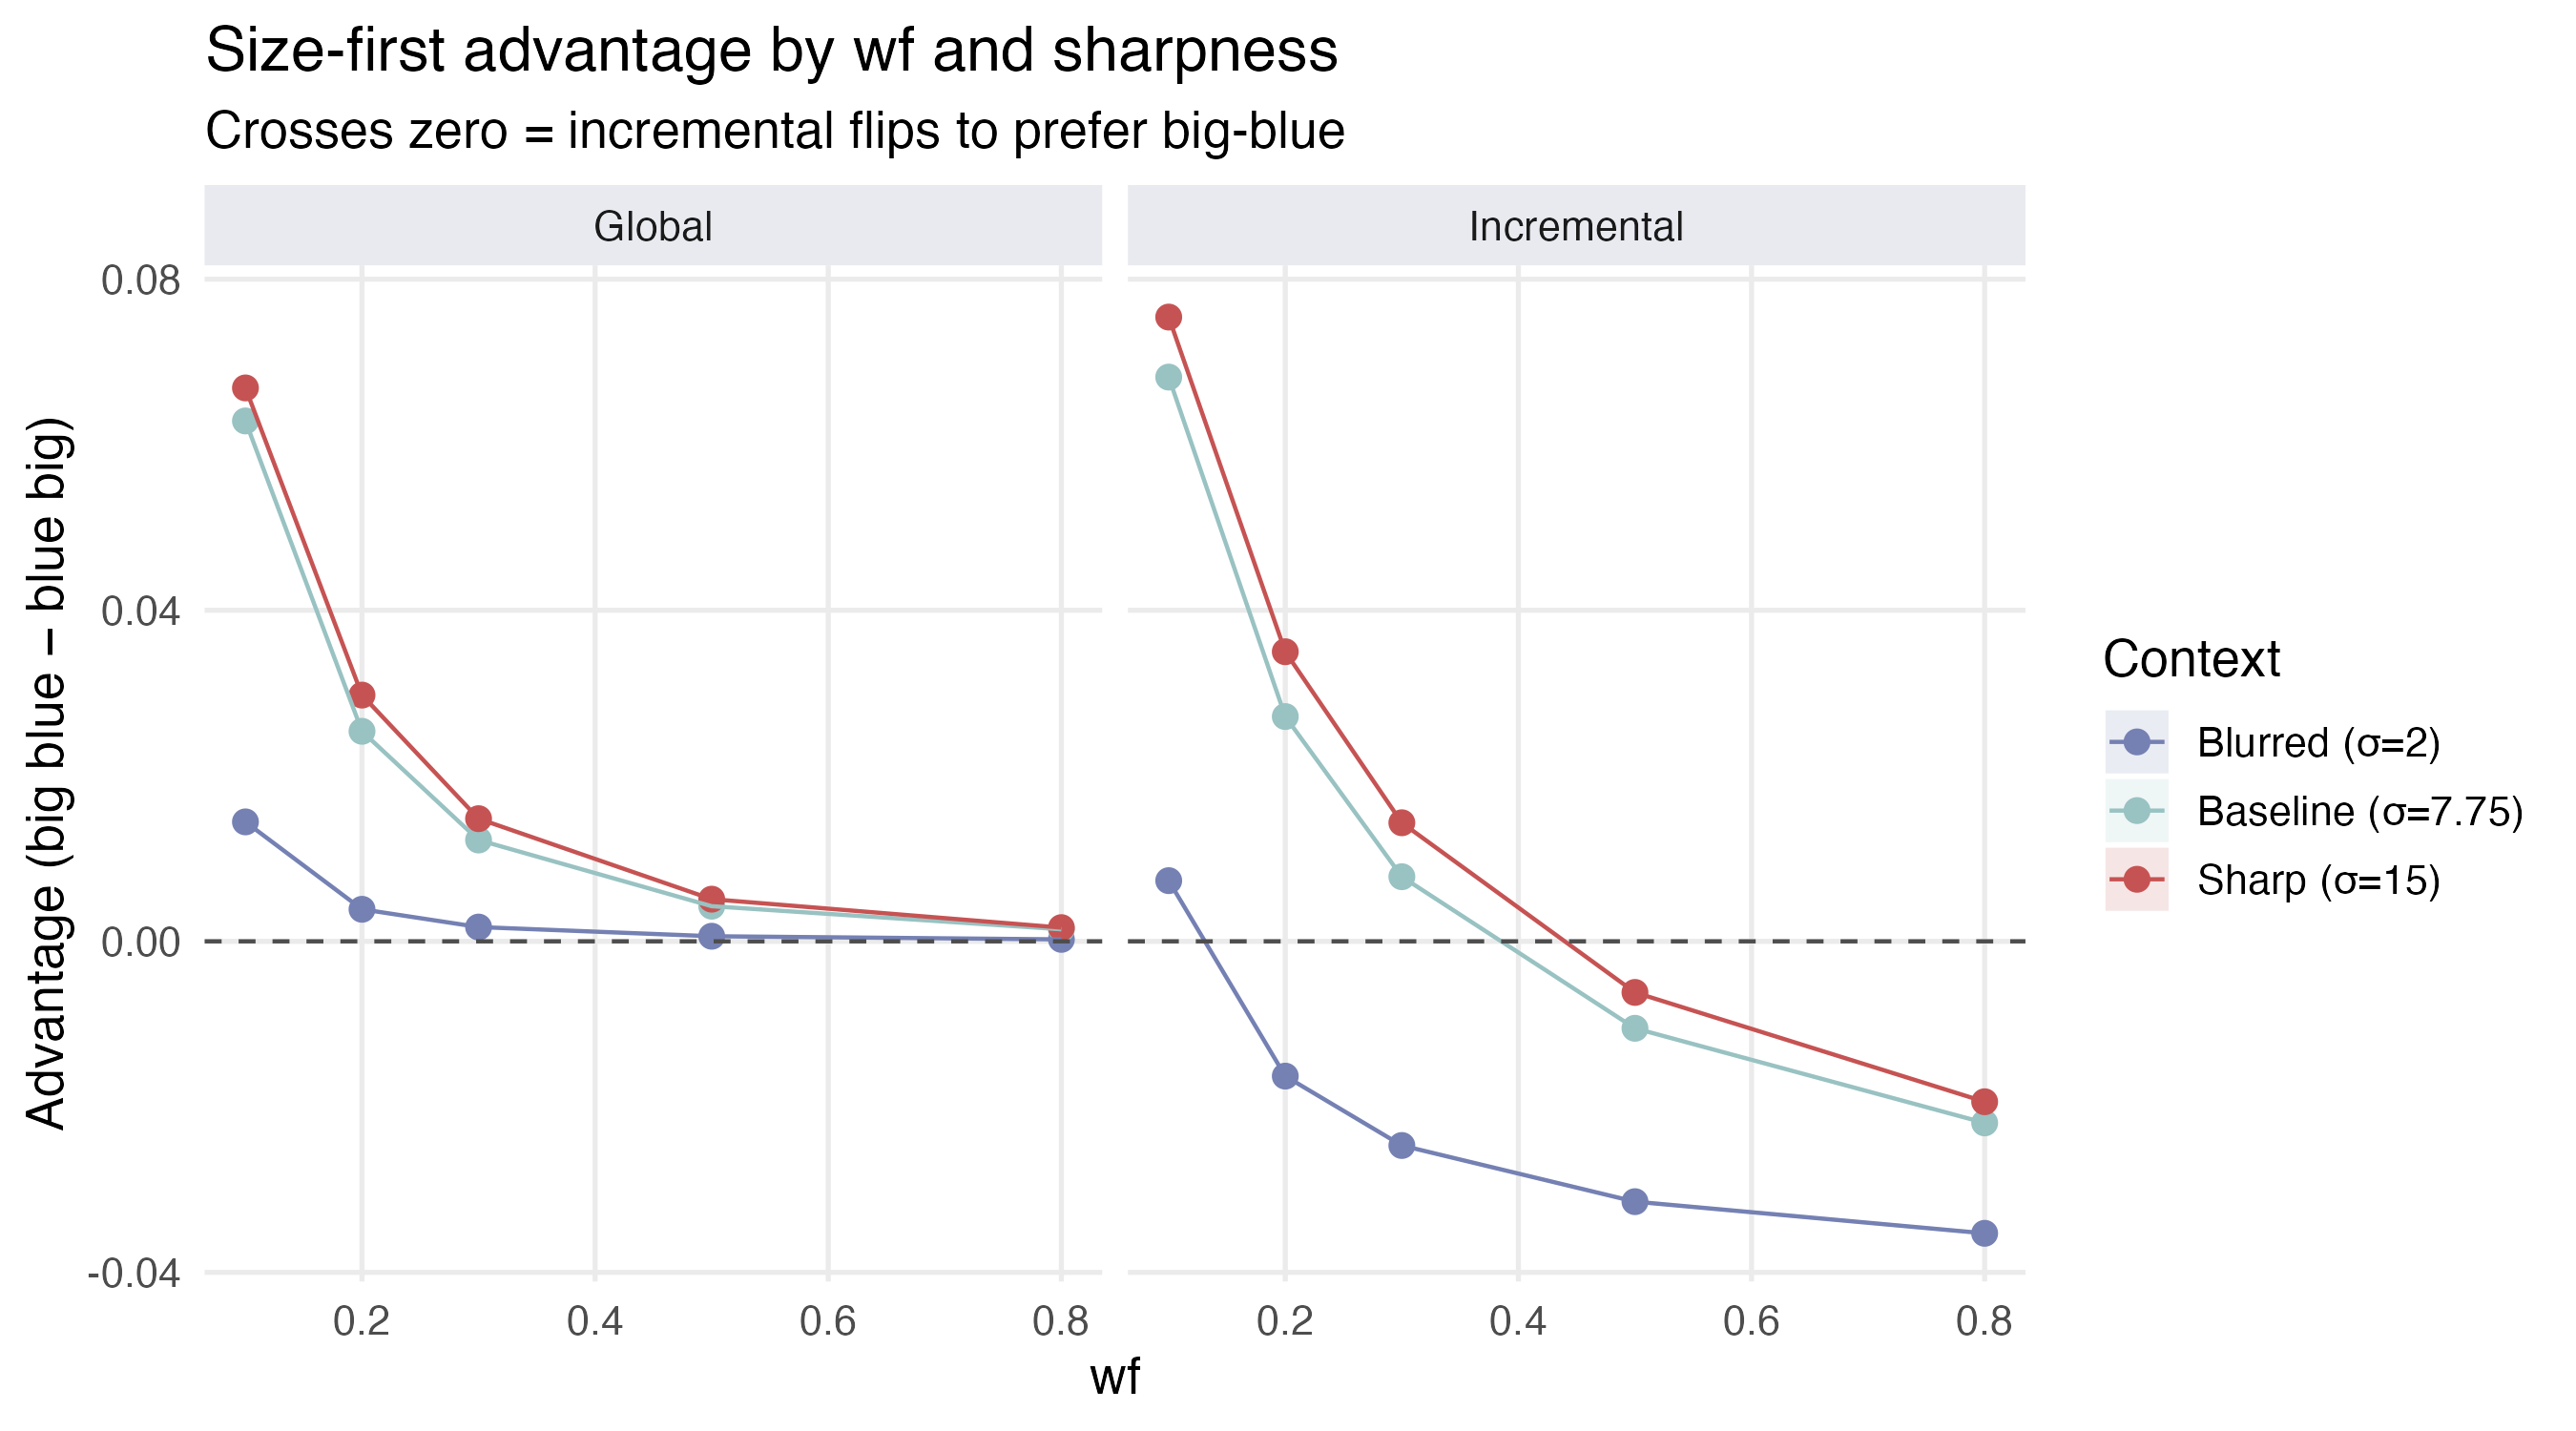
\includegraphics[width=\columnwidth]{../04-simulation-w-randomstates/sim_advantage_wf_sd.png}
  \caption{Mean size-first advantage ($\Delta$) as a function of perceptual
    blur $\omega$ for incremental and global speakers under recursive
    semantics, broken down by context sharpness $\sigma_{\text{sd}}$.
    Error bands show $\pm 2$ SE.
    The dashed line marks $\Delta = 0$.
    The global speaker is insensitive to $\omega$; the incremental speaker
    crosses from negative to positive at $\omega \approx 0.30$.}
  \label{fig:adv-wf}
\end{figure}

Table~\ref{tab:wf-sd} reports mean $\Delta$ at each combination of
$\omega$ and $\sigma_{\text{sd}}$ for the incremental speaker under
recursive semantics.
At $\omega = 0.1$, sharp contexts ($\sigma_{\text{sd}} = 15$) produce
$\Delta = +0.074$, approximately five times the global-speaker advantage,
while blurred contexts ($\sigma_{\text{sd}} = 2$) yield only $+0.006$.
This interaction occurs because a sharp context distributes objects
across a wide size range, making the size adjective highly diagnostic
when $\omega$ is small.
In a blurred context, objects cluster near a common size, and even a
steep CDF cannot make ``big'' much more discriminating than chance.

\begin{table}[h]
\centering
\small
\caption{Mean size-first advantage $\Delta$ for the incremental speaker
  under recursive semantics,
  by perceptual blur $\omega$ and context sharpness $\sigma_{\text{sd}}$.}
\label{tab:wf-sd}
\begin{tabular}{lccc}
\toprule
 & \multicolumn{3}{c}{$\sigma_{\text{sd}}$} \\
\cmidrule(lr){2-4}
$\omega$ & 2.0 & 7.75 & 15.0 \\
\midrule
0.1 & $+0.006$ & $+0.067$ & $+0.074$ \\
0.2 & $-0.017$ & $+0.027$ & $+0.034$ \\
0.3 & $-0.025$ & $+0.007$ & $+0.014$ \\
0.5 & $-0.032$ & $-0.011$ & $-0.005$ \\
0.8 & $-0.036$ & $-0.022$ & $-0.018$ \\
\bottomrule
\end{tabular}
\end{table}

\subsubsection{Static Semantics Eliminates the Global Advantage}

The most striking result of the $2 \times 2$ design is that static
semantics completely eliminates the global speaker's size-first advantage.
Under static semantics, the global speaker produced $\Delta = 0.000$
across all parameter combinations without exception.
This occurs because, when the size threshold is held fixed at the
uniform-prior value, the literal listener produces identical posterior
distributions for \textit{big blue} and \textit{blue big}: both orderings
compose the same semantic values over the same prior, differing only in
application order, which is irrelevant when the threshold does not update.
The global speaker, which selects between complete utterances based on
their literal-listener informativeness, therefore assigns equal probability
to both orderings for every referent.

The incremental speaker under static semantics produced a mean advantage
of $\Delta = -0.009$, with only 33.6\% of parameter combinations favoring
size-first — a stronger color-first bias than under recursive semantics
($\Delta = +0.004$).
Without recursive threshold adaptation, the size adjective is less
diagnostic at step~1, amplifying the chain-rule asymmetry that favors
``blue'' as the opening token.

\subsubsection{Role of the Threshold Parameter $k$}

The threshold parameter $k$ has opposite directional effects on the two
speaker architectures under recursive semantics.
For the incremental speaker, higher $k$ (lower threshold; more objects
qualify as ``big'') degrades size-first advantage — increasing $k$ from
0.1 to 0.9 reduces the mean advantage by approximately 0.019 — because a
permissive threshold weakens the discriminating power of ``big.''
For the global speaker, the same manipulation leaves the advantage
virtually unchanged.
Under static semantics, $k$ has no effect on the global speaker (the
advantage is zero everywhere) and amplifies the color-first bias for the
incremental speaker.

\subsubsection{Effect of Context Size}

Figure~\ref{fig:nobj-2x2} shows the size-first advantage as a function
of $n_{\text{obj}}$, faceted by speaker model and semantic regime.
Under recursive semantics (top row), both speakers show their largest
advantages at small $n_{\text{obj}}$, with $\Delta$ converging toward
zero as the context grows and referent probability is diluted across
more objects.
The direction of the advantage is preserved across context sizes for
the global speaker.
For the incremental speaker the direction is parameter-dependent, but
the crossover at $\omega \approx 0.30$ is robust to $n_{\text{obj}}$.

Under static semantics (bottom row), the global speaker shows zero
advantage at all context sizes.
The incremental speaker shows a negative advantage (color-first), most
pronounced at small $n_{\text{obj}}$ with blurred contexts, converging
toward zero as the context grows.

\begin{figure}[h]
  \centering
  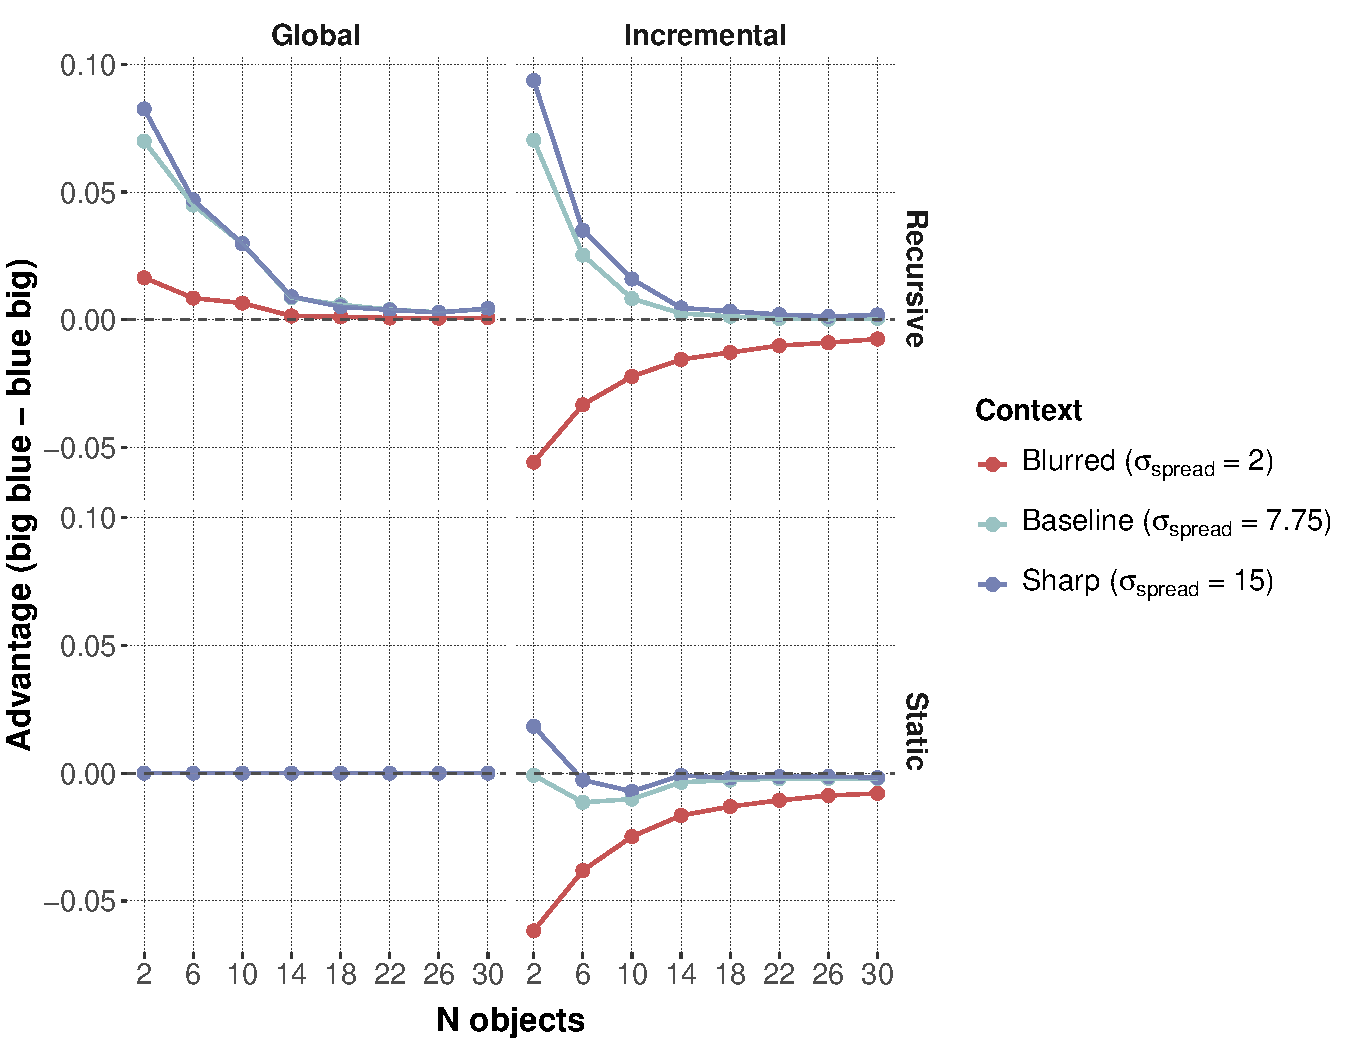
\includegraphics[width=\columnwidth]{figures/sim_advantage_nobj.pdf}
  \caption{Mean size-first advantage ($\Delta$) as a function of context
    size $n_{\text{obj}}$, faceted by speaker model (columns) and semantic
    regime (rows).
    Lines show context sharpness $\sigma_{\text{sd}}$.
    Error bands show $\pm 2$ SE.
    Under static semantics the global speaker produces zero advantage at
    all context sizes; the incremental speaker shows a negative (color-first)
    bias that diminishes with context size.}
  \label{fig:nobj-2x2}
\end{figure}

\subsection{Summary}

The $2 \times 2$ simulation reveals that both speaker architecture and
semantic regime are necessary to predict canonical adjective ordering.
Recursive semantics is required for the global speaker to produce any
size-first advantage at all: under static semantics the two orderings
are informationally equivalent.
The incremental speaker can produce a size-first advantage under
recursive semantics when perceptual blur is low
($\omega \lesssim 0.30$) and context sharpness is high, but defaults
to color-first under static semantics across most of the parameter space.
The critical interaction is between semantic regime and speaker
architecture: recursive semantics creates an asymmetry in the literal
listener that the global speaker exploits directly and that the
incremental speaker can leverage when size is sufficiently diagnostic
at step~1.
These results motivate estimating $\omega$ from empirical
adjective-ordering data rather than fixing it a priori, and they
highlight recursive semantics as a key architectural choice whose
contribution can be isolated from the speaker's composition strategy.

% =============================================================================

\section{Simulation}

\subsection{Overview}

A factorial simulation examined how two RSA speaker architectures and two
semantic regimes jointly determine the size-first advantage.
The speaker factor crosses an \textit{incremental} speaker that composes
utterances token-by-token via a chain rule with a \textit{global} speaker
that evaluates full two-word utterances at once.
The semantics factor crosses \textit{recursive} semantics, in which the
size threshold adapts to the listener's running posterior at each
composition step, with \textit{static} semantics, in which the threshold is
computed once from the uniform prior and held fixed.
The central measure is communicative success: the probability that a
pragmatic listener, reasoning about the speaker, recovers the intended
referent from a given utterance.
Size-first (\textit{big blue}) is taken to be preferred whenever it yields
strictly higher communicative success than color-first (\textit{blue big}).

\subsection{Model}

\paragraph{Referents and contexts.}
Each context consists of $n_{\text{obj}}$ objects drawn from a
log-normal size distribution with spread parameter $\sigma_{\text{sd}}$,
with each draw independently assigned a uniformly random color (0 or 1) and
form (0 or 1).
The intended referent is always the object with the largest size, color
$= 1$ (``blue''), and form $= 1$.
The uniform object prior is $P(s) = 1/n_{\text{obj}}$.

\paragraph{Adjective semantics.}
For a color adjective (``blue''),
\begin{equation}
  \llbracket \text{blue} \rrbracket(s) \;=\;
  c_s \cdot v_c + (1 - c_s)(1 - v_c),
\end{equation}
where $c_s \in \{0,1\}$ is the object's color feature and
$v_c \in (0.5, 1)$ is the color semantic value (how reliably the word
maps to the feature).

For a size adjective (``big''), applicability is modeled as a
cumulative-normal threshold function with perceptual blur $\omega$:
\begin{equation}
  \llbracket \text{big} \rrbracket(s) \;=\;
  \Phi\!\left(\frac{s - \theta}{\omega\sqrt{s^2 + \theta^2}}\right),
\end{equation}
where $\theta$ is a context-sensitive threshold and
$\omega$ controls sharpness: small $\omega$ produces a steep CDF
so that only the very largest object receives high applicability.

\paragraph{Threshold.}
The threshold $\theta$ is defined over the mid-range of the context
distribution $C$,
\begin{equation}
  \theta_k(C) \;=\;
  x_{\max}^{\text{mid}}(C) - k\bigl(x_{\max}^{\text{mid}}(C) - x_{\min}^{\text{mid}}(C)\bigr),
\end{equation}
where $x_{\min}^{\text{mid}}$ and $x_{\max}^{\text{mid}}$ are the
20th- and 80th-percentile sizes in $C$, and $k \in [0,1]$ shifts
the threshold between the top and the middle of the mid-range.
Higher $k$ lowers the threshold, admitting more objects as ``big.''

\paragraph{Literal listener.}
For single-word utterances,
$L_0(s \mid w) \propto \llbracket w \rrbracket(s) \cdot P(s)$.
For two-word utterances $u = w_1 w_2$, the literal listener applies
backward functional composition, processing tokens right-to-left and
updating the posterior at each step.
Under \textit{recursive} semantics, the size threshold $\theta$ is
recomputed from this running posterior before each token is applied, so the
threshold adapts to the listener's evolving belief state.
Under \textit{static} semantics, $\theta$ is computed once from the uniform
prior and held fixed throughout composition.
In both cases the final result is
$L_0(s \mid w_1 w_2) \propto
  \llbracket w_1 \rrbracket(s) \cdot \llbracket w_2 \rrbracket(s) \cdot P(s)$,
but under recursive semantics the semantic values of the size adjective
differ between the two orderings because the threshold depends on which
token was processed first.

\paragraph{Global speaker.}
The global speaker evaluates both full two-word utterances simultaneously,
\begin{equation}
  S_G(u \mid s) \;\propto\; \bigl[L_0(s \mid u)\bigr]^\alpha,
  \quad u \in \{\text{big-blue},\; \text{blue-big}\},
\end{equation}
treating each ordering as an atomic unit.

\paragraph{Incremental speaker.}
The incremental speaker applies a two-step chain rule
following \citeA{cohn-gordon-et-al2019}.
At step 1, it selects a first token by reasoning over the single-word
literal listener:
\begin{equation}
  S_1(w_1 \mid s)
    \;\propto\; \bigl[L_0(s \mid w_1)\bigr]^\alpha.
\end{equation}
At step 2, given prefix $w_1$, it decides whether to continue:
\begin{equation}
  S_2(w_2 \mid w_1, s)
    \;\propto\; \bigl[L_0(s \mid w_1 w_2)\bigr]^\alpha,
\end{equation}
where the alternative is stopping at the single word $w_1$.
The full utterance probability is then
\begin{equation}
  S_I(w_1 w_2 \mid s) \;=\; S_1(w_1 \mid s) \cdot S_2(w_2 \mid w_1, s).
  \label{eq:inc-chain}
\end{equation}

\paragraph{Pragmatic listener.}
The pragmatic listener inverts the speaker distribution via Bayes' rule
with a uniform prior over referents,
\begin{equation}
  L_1(s \mid u) \;\propto\; S(u \mid s) \cdot P(s).
\end{equation}
The primary dependent variable is the \textit{size-first advantage},
\begin{equation}
  \Delta(s) \;=\;
  L_1(s^* \mid \text{big-blue}) - L_1(s^* \mid \text{blue-big}),
\end{equation}
where $s^*$ is the intended referent.
Positive values indicate that the size-first order yields higher
communicative success.

\subsection{Parameter Sweep}

Seven parameters were varied factorially (Table~\ref{tab:params}).
For each combination, 1{,}000 contexts were sampled, yielding
12{,}000{,}000 rows total.
The simulation was implemented in JAX \citep{jax2018github} and executed
in a single vectorized pass using nested \texttt{vmap}/\texttt{jit},
completing in under 90 seconds on CPU.

\begin{table}[h]
\centering
\small
\caption{Simulation parameter grid.}
\label{tab:params}
\begin{tabular}{llc}
\toprule
Parameter & Values & $n$ \\
\midrule
$n_{\text{obj}}$    & 2, 6, 10, 14, 18, 22, 26, 30 & 8 \\
Speaker model       & incremental, global           & 2 \\
Semantics           & recursive, static             & 2 \\
$v_c$ (color sem.)  & 0.90, 0.92, 0.94, 0.96, 0.98 & 5 \\
$k$ (threshold)     & 0.1, 0.3, 0.5, 0.7, 0.9      & 5 \\
$\omega$ (blur)     & 0.1, 0.2, 0.3, 0.5, 0.8      & 5 \\
$\sigma_{\text{sd}}$ (context spread) & 2.0, 7.75, 15.0 & 3 \\
\midrule
\multicolumn{2}{l}{Fixed: $\alpha = 1$, bias $= 0$, utterance length $= 2$} & \\
\bottomrule
\end{tabular}
\end{table}

\subsection{Results}

\subsubsection{Recursive Semantics: Global Speaker}

Under recursive semantics, the global speaker produced a consistent
size-first advantage across virtually all parameter combinations.
Averaging over all contexts and parameter values, it assigned
$L_1(s^* \mid \text{big-blue}) = 0.138$ versus
$L_1(s^* \mid \text{blue-big}) = 0.122$,
yielding a mean advantage of $\Delta = +0.016$.
Across individual parameter combinations, 64.8\% produced a positive
advantage, and the direction was preserved across all levels of
$n_{\text{obj}}$, $\sigma_{\text{sd}}$, and $v_c$.

The preference arises because, under recursive semantics, the size
threshold shifts when ``big'' versus ``blue'' is processed first.
This asymmetry in the literal listener makes the two orderings
non-equivalent, and the global speaker exploits the ordering that
maximizes referent recovery.

\subsubsection{Recursive Semantics: Incremental Speaker}

Under recursive semantics, the incremental speaker showed a qualitatively
different pattern depending on the perceptual blur parameter $\omega$.
At $\omega = 0.5$ (the default in prior work), the incremental speaker
produced a \textit{negative} mean advantage ($\Delta = -0.016$),
with only 23.7\% of parameter combinations favoring size-first.
This reversal reflects a structural asymmetry in the chain rule
(Equation~\ref{eq:inc-chain}):
The referent is by construction the only object with color $= 1$, so
$\llbracket \text{blue} \rrbracket(s^*)$ is close to $v_c$ ($\approx 0.90$--$0.98$)
while $\llbracket \text{blue} \rrbracket(s)$ for any non-referent is close to
$1 - v_c$ ($\approx 0.02$--$0.10$).
The color adjective thus almost perfectly identifies the referent at
step~1.
The size adjective, however, depends on $\omega$: at large $\omega$,
the CDF is shallow and multiple objects receive moderate size
applicability, reducing the discriminating power of ``big'' relative to
``blue.''
When ``blue'' is the more informative first token, the incremental
speaker prefers to say it first, producing \textit{blue big}.

Reducing $\omega$ sharpens the size CDF so that only the largest object
receives high applicability, restoring size as a reliable discriminator at
step~1.
Figure~\ref{fig:adv-wf} shows a monotone relationship between $\omega$
and $\Delta$ for the incremental speaker: the size-first advantage crosses
zero at approximately $\omega \approx 0.30$, and reaches a mean of
$+0.049$ at $\omega = 0.1$.

\begin{figure}[h]
  \centering
  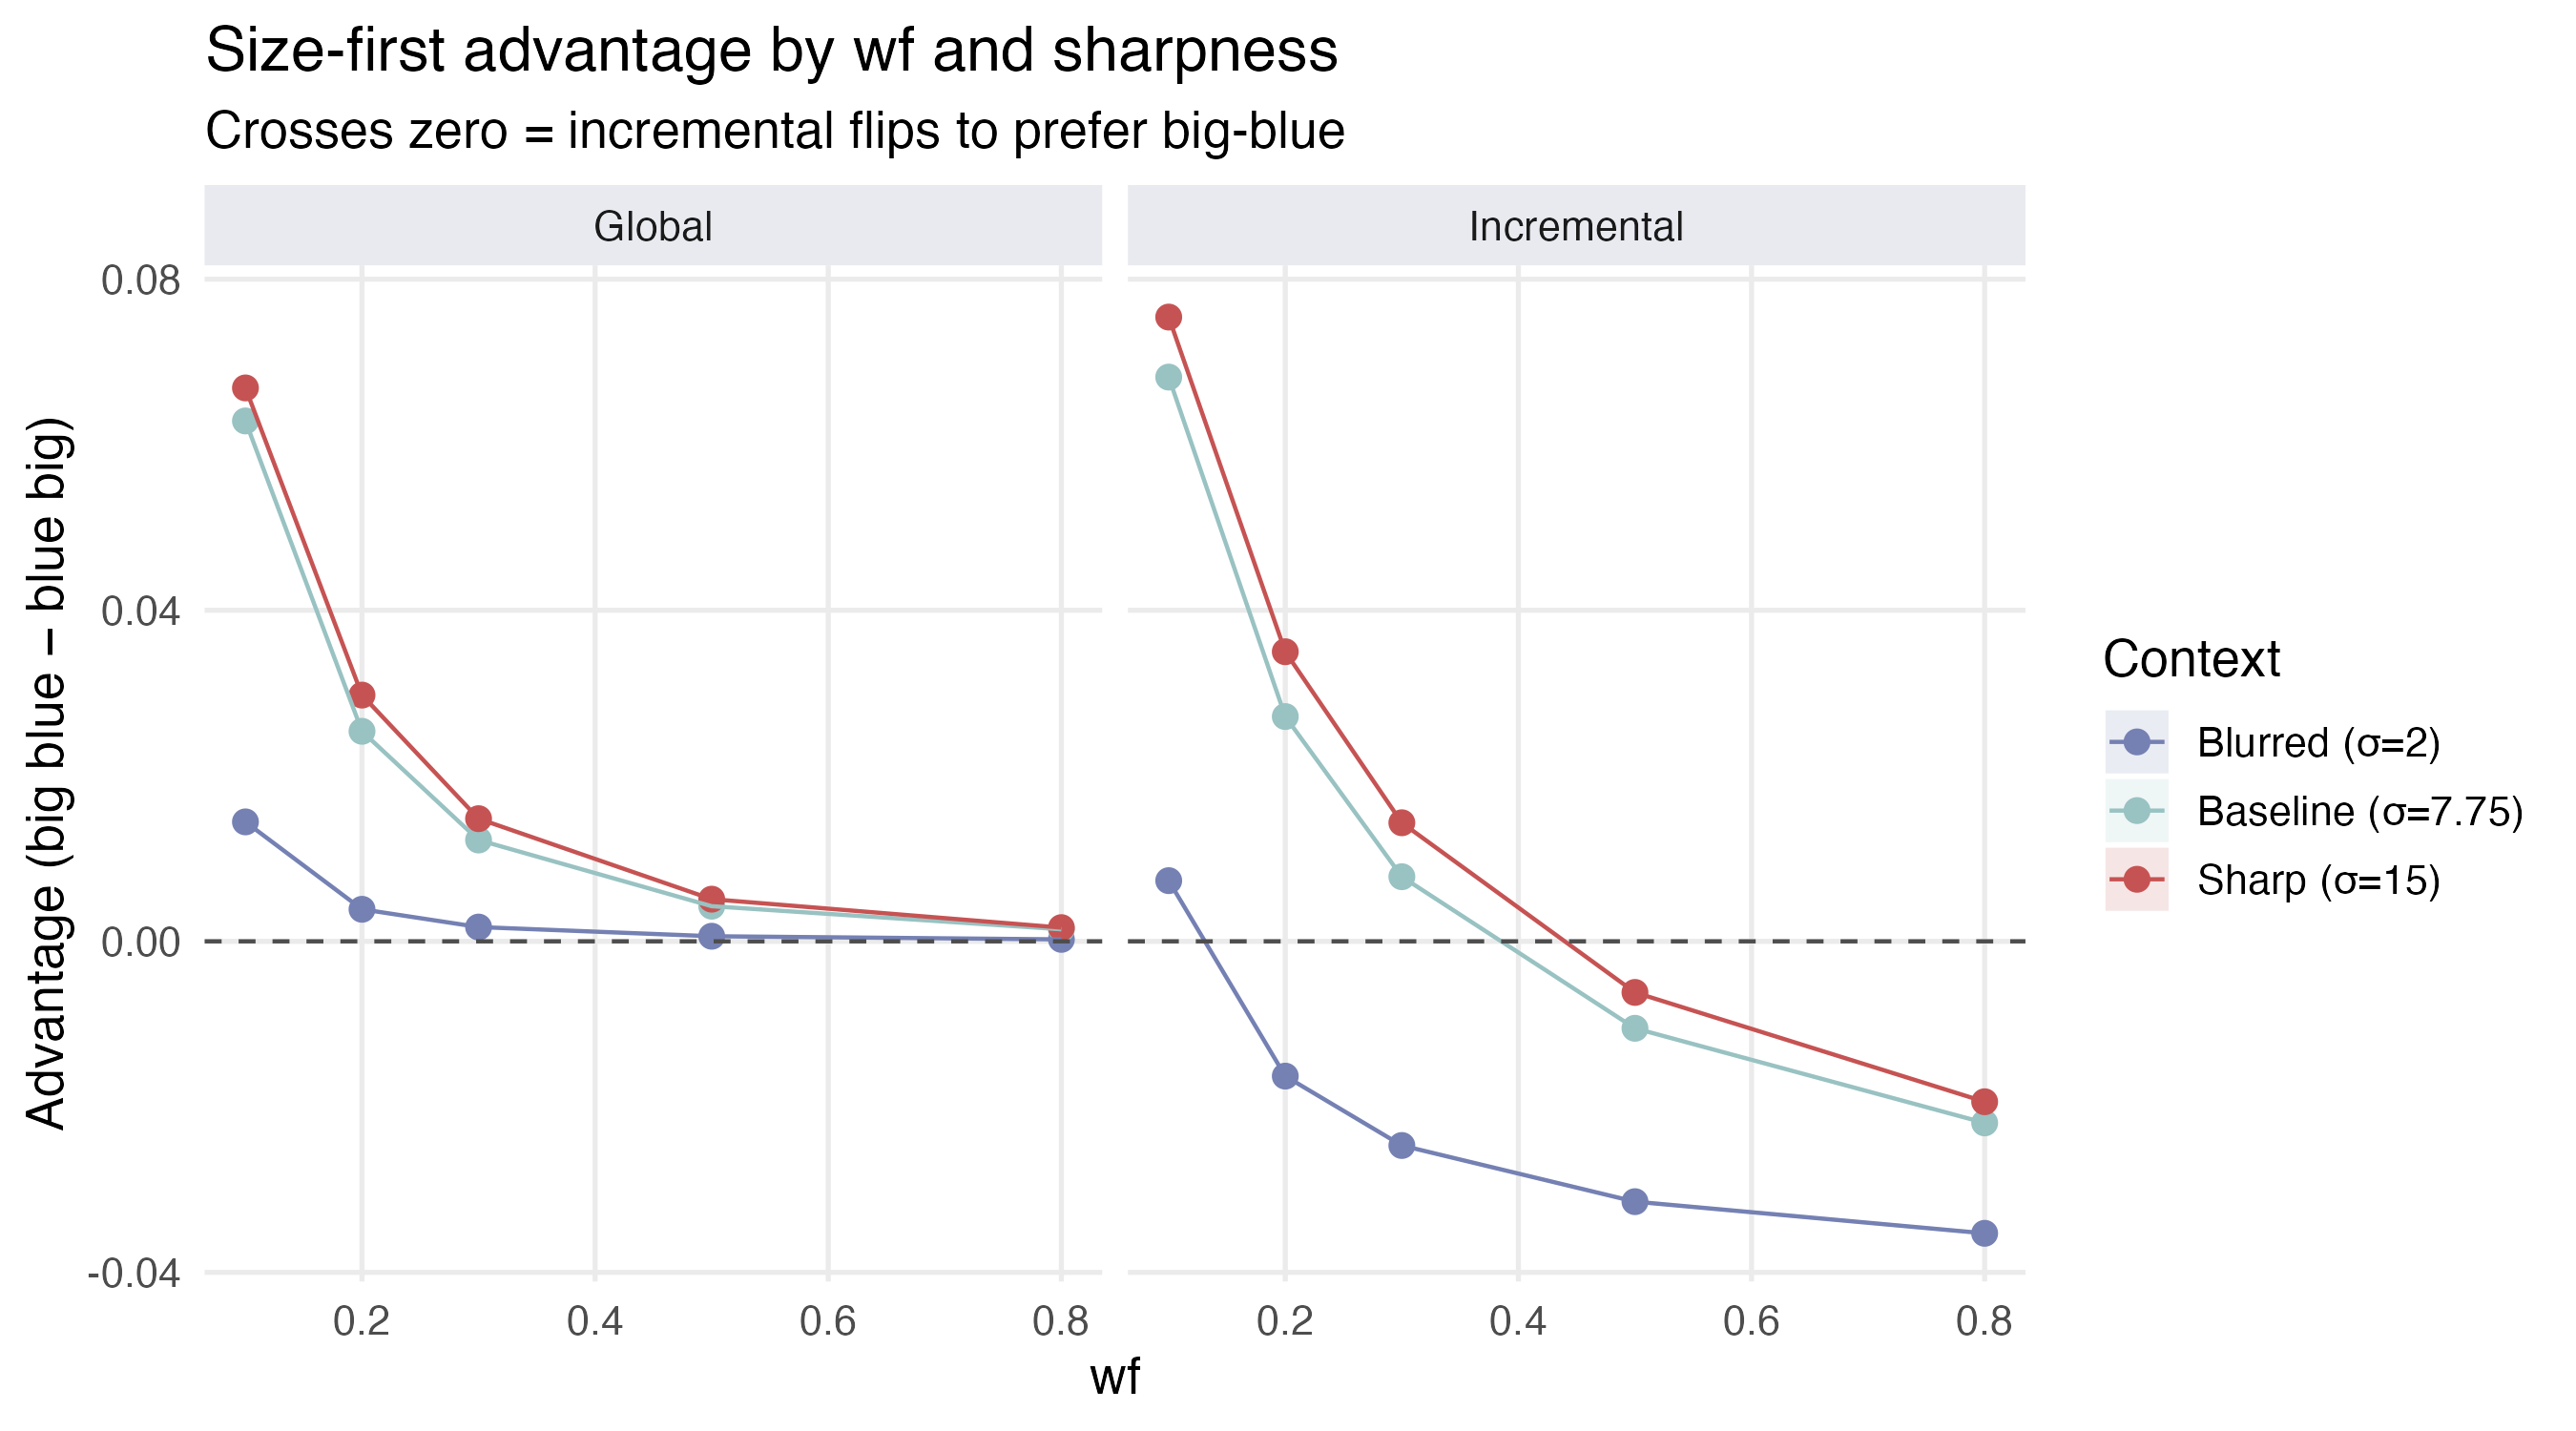
\includegraphics[width=\columnwidth]{../04-simulation-w-randomstates/sim_advantage_wf_sd.png}
  \caption{Mean size-first advantage ($\Delta$) as a function of perceptual
    blur $\omega$ for incremental and global speakers under recursive
    semantics, broken down by context sharpness $\sigma_{\text{sd}}$.
    Error bands show $\pm 2$ SE.
    The dashed line marks $\Delta = 0$.
    The global speaker is insensitive to $\omega$; the incremental speaker
    crosses from negative to positive at $\omega \approx 0.30$.}
  \label{fig:adv-wf}
\end{figure}

Table~\ref{tab:wf-sd} reports mean $\Delta$ at each combination of
$\omega$ and $\sigma_{\text{sd}}$ for the incremental speaker under
recursive semantics.
At $\omega = 0.1$, sharp contexts ($\sigma_{\text{sd}} = 15$) produce
$\Delta = +0.074$, approximately five times the global-speaker advantage,
while blurred contexts ($\sigma_{\text{sd}} = 2$) yield only $+0.006$.
This interaction occurs because a sharp context distributes objects
across a wide size range, making the size adjective highly diagnostic
when $\omega$ is small.
In a blurred context, objects cluster near a common size, and even a
steep CDF cannot make ``big'' much more discriminating than chance.

\begin{table}[h]
\centering
\small
\caption{Mean size-first advantage $\Delta$ for the incremental speaker
  under recursive semantics,
  by perceptual blur $\omega$ and context sharpness $\sigma_{\text{sd}}$.}
\label{tab:wf-sd}
\begin{tabular}{lccc}
\toprule
 & \multicolumn{3}{c}{$\sigma_{\text{sd}}$} \\
\cmidrule(lr){2-4}
$\omega$ & 2.0 & 7.75 & 15.0 \\
\midrule
0.1 & $+0.006$ & $+0.067$ & $+0.074$ \\
0.2 & $-0.017$ & $+0.027$ & $+0.034$ \\
0.3 & $-0.025$ & $+0.007$ & $+0.014$ \\
0.5 & $-0.032$ & $-0.011$ & $-0.005$ \\
0.8 & $-0.036$ & $-0.022$ & $-0.018$ \\
\bottomrule
\end{tabular}
\end{table}

\subsubsection{Static Semantics Eliminates the Global Advantage}

The most striking result of the $2 \times 2$ design is that static
semantics completely eliminates the global speaker's size-first advantage.
Under static semantics, the global speaker produced $\Delta = 0.000$
across all parameter combinations without exception.
This occurs because, when the size threshold is held fixed at the
uniform-prior value, the literal listener produces identical posterior
distributions for \textit{big blue} and \textit{blue big}: both orderings
compose the same semantic values over the same prior, differing only in
application order, which is irrelevant when the threshold does not update.
The global speaker, which selects between complete utterances based on
their literal-listener informativeness, therefore assigns equal probability
to both orderings for every referent.

The incremental speaker under static semantics produced a mean advantage
of $\Delta = -0.009$, with only 33.6\% of parameter combinations favoring
size-first — a stronger color-first bias than under recursive semantics
($\Delta = +0.004$).
Without recursive threshold adaptation, the size adjective is less
diagnostic at step~1, amplifying the chain-rule asymmetry that favors
``blue'' as the opening token.

\subsubsection{Role of the Threshold Parameter $k$}

The threshold parameter $k$ has opposite directional effects on the two
speaker architectures under recursive semantics.
For the incremental speaker, higher $k$ (lower threshold; more objects
qualify as ``big'') degrades size-first advantage — increasing $k$ from
0.1 to 0.9 reduces the mean advantage by approximately 0.019 — because a
permissive threshold weakens the discriminating power of ``big.''
For the global speaker, the same manipulation leaves the advantage
virtually unchanged.
Under static semantics, $k$ has no effect on the global speaker (the
advantage is zero everywhere) and amplifies the color-first bias for the
incremental speaker.

\subsubsection{Effect of Context Size}

Figure~\ref{fig:nobj-2x2} shows the size-first advantage as a function
of $n_{\text{obj}}$, faceted by speaker model and semantic regime.
Under recursive semantics (top row), both speakers show their largest
advantages at small $n_{\text{obj}}$, with $\Delta$ converging toward
zero as the context grows and referent probability is diluted across
more objects.
The direction of the advantage is preserved across context sizes for
the global speaker.
For the incremental speaker the direction is parameter-dependent, but
the crossover at $\omega \approx 0.30$ is robust to $n_{\text{obj}}$.

Under static semantics (bottom row), the global speaker shows zero
advantage at all context sizes.
The incremental speaker shows a negative advantage (color-first), most
pronounced at small $n_{\text{obj}}$ with blurred contexts, converging
toward zero as the context grows.

\begin{figure}[h]
  \centering
  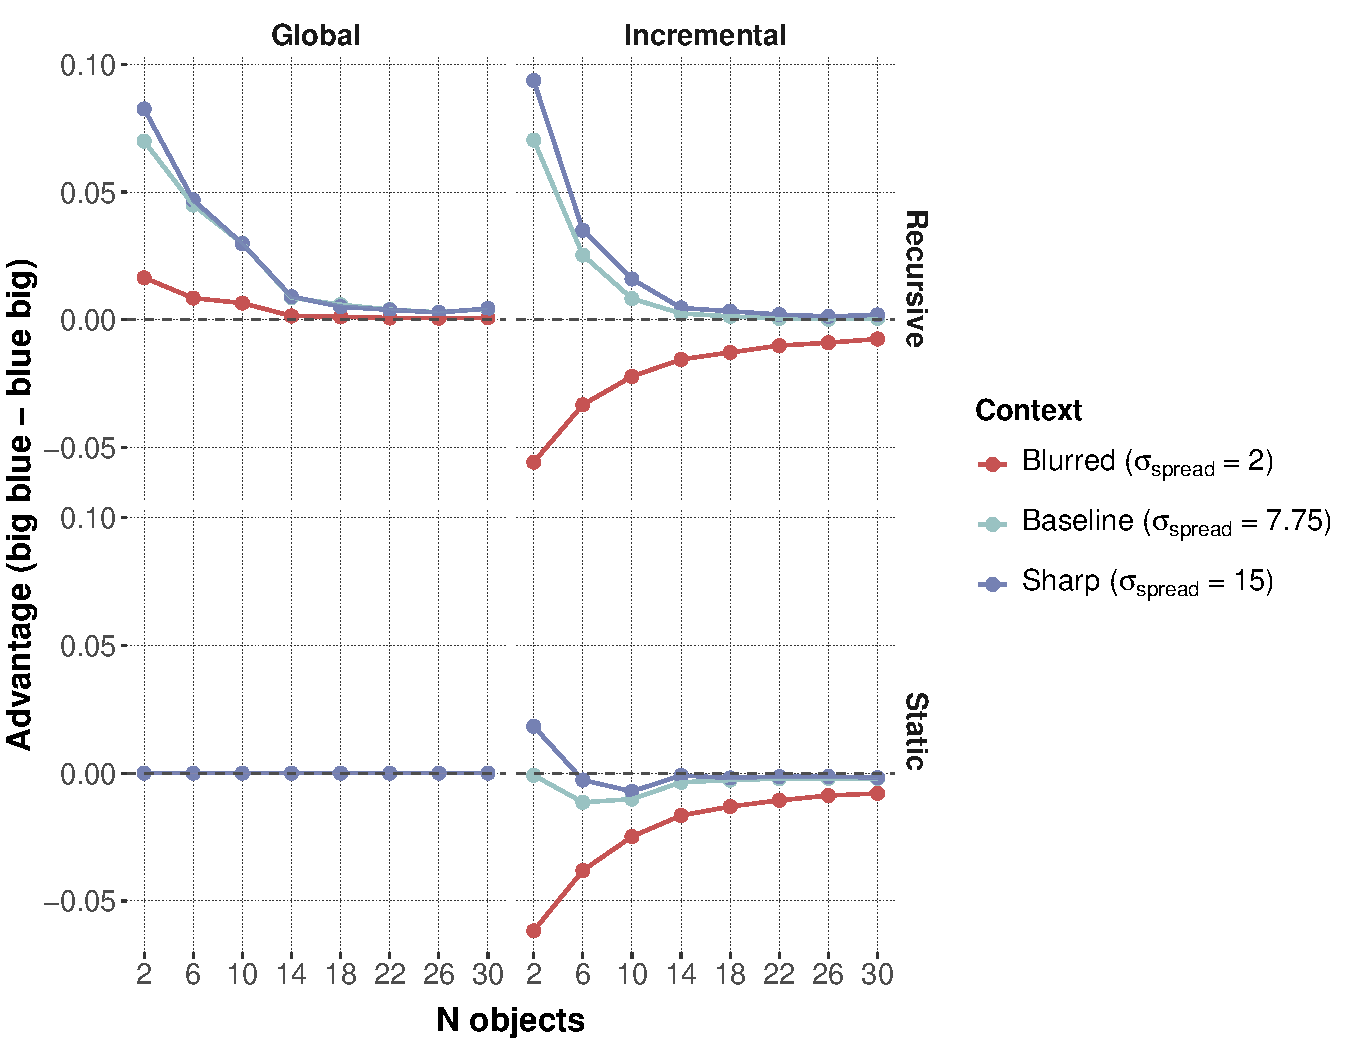
\includegraphics[width=\columnwidth]{figures/sim_advantage_nobj.pdf}
  \caption{Mean size-first advantage ($\Delta$) as a function of context
    size $n_{\text{obj}}$, faceted by speaker model (columns) and semantic
    regime (rows).
    Lines show context sharpness $\sigma_{\text{sd}}$.
    Error bands show $\pm 2$ SE.
    Under static semantics the global speaker produces zero advantage at
    all context sizes; the incremental speaker shows a negative (color-first)
    bias that diminishes with context size.}
  \label{fig:nobj-2x2}
\end{figure}

\subsection{Summary}

The $2 \times 2$ simulation reveals that both speaker architecture and
semantic regime are necessary to predict canonical adjective ordering.
Recursive semantics is required for the global speaker to produce any
size-first advantage at all: under static semantics the two orderings
are informationally equivalent.
The incremental speaker can produce a size-first advantage under
recursive semantics when perceptual blur is low
($\omega \lesssim 0.30$) and context sharpness is high, but defaults
to color-first under static semantics across most of the parameter space.
The critical interaction is between semantic regime and speaker
architecture: recursive semantics creates an asymmetry in the literal
listener that the global speaker exploits directly and that the
incremental speaker can leverage when size is sufficiently diagnostic
at step~1.
These results motivate estimating $\omega$ from empirical
adjective-ordering data rather than fixing it a priori, and they
highlight recursive semantics as a key architectural choice whose
contribution can be isolated from the speaker's composition strategy.
